\documentclass[openany]{book}
\title{LaTeX Notes}
\author{Alpha Huang}
\date{\today}
\usepackage{subfigure}
\usepackage{array}
\usepackage{booktabs}%三线表
\usepackage[T1]{fontenc}
\usepackage{here}
\usepackage{enumerate}   
\usepackage[utf8]{inputenc}
\usepackage[a4paper,left=4cm,right=3cm,top=3cm,bottom=3cm,
]{geometry}
\usepackage[english]{babel}
\usepackage{biblatex} %Imports biblatex package
\addbibresource{sample.bib} %Import the bibliography file
\usepackage{amsmath}
\usepackage{graphicx}
\usepackage{titlesec}
\titleformat{\chapter}[hang] 
{\largefont\huge\bfseries}{\chaptertitlename \vspace{0.5em} \thechapter}{1em}{}
\usepackage{indentfirst}
%paragraph indentation
\setlength{\parindent}{2em}
%paragraph spacing
\addtolength{\parskip}{3pt}
%Line spacing

\usepackage[justification=centering]{caption}
%centering caption of a figure

\renewcommand{\baselinestretch}{1.15}
\graphicspath{ {./fig/} }
\usepackage{float}

\usepackage{fancyhdr}%没有页眉,页脚中部放置页码
\pagestyle{plain}

\begin{document}
\maketitle
\tableofcontents
\let\cleardoublepage\clearpage
\chapter*{Background}
The portable energy sources, such as rechargeable batteries, supercapacitors, and fuel cells, are critical to economic development and human's daily life. Among the several types of rechargeable batteries, lithium-ion batteries (LIBs) are the most promising for their highest performance: high energy density; long cycle life; low rate of self-discharge; environmental pollution. Besides, LIBs are also more flexible in terms of design for a wide range of applications in portable electronic devices, being able to be manufactured in numerous sizes and shapes to make effective use of spaces. Since the commercialization of LIBs in 1991, LIBs have been utilized in laptops, cellar phones, and even larger-scale electric vehicles (EVs). 

Especially, to tackle the dilemma of rapid fossil fuel depletion and environmental pollution, governments all around the world have introduced policies to implement the transition from a fossil-based economy to a zero-carbon economy in the next decade, making the EVs crucial to realize such transition. Therefore, the EVs sales worldwide have soared in recent five years. In 2010, only about 17,000 electric cars were on the world’s roads. But by 2019, that number has swelled to 7.2 million, 47\% of which are in China. The future EVs market is of great potential.
However, the further commercialization of EVs is still hindered by several technological barriers principally from LIBs, including high costs, insufficient cycle lives, intrinsically poor safety characteristics, and poor performances at low temperatures.  

Based on the above background, this study focus on investigating next generation LIBs from a material's point of view.

\chapter{Introduction}
\section{Lithium ion battery (LIB)}
\subsection{The features of LIB\textsuperscript{[1]}}
Primary Li batteries were invented in the 1970s by M. Stanley Whittingham and then developed by John B. Goodenough and Akira Yoshino[1]. LIBs have been one of the most predominant power sources ever since 1991. Compared to other secondary batteries such as Nickel-Cadmium battery (NiCd), Nickel-metal battery (Ni-M), LiBs are featured with the highest energy density, higher operating voltages, limited self-discharging, long cycle life, lower maintenance requirements, and environmental friendliness. Also, it is well known that they do not suffer from ‘memory’ effects that plague other batteries. These matchless advantages make LIBs commonplace in secondary battery market. 
\begin{figure}[h]
\centering
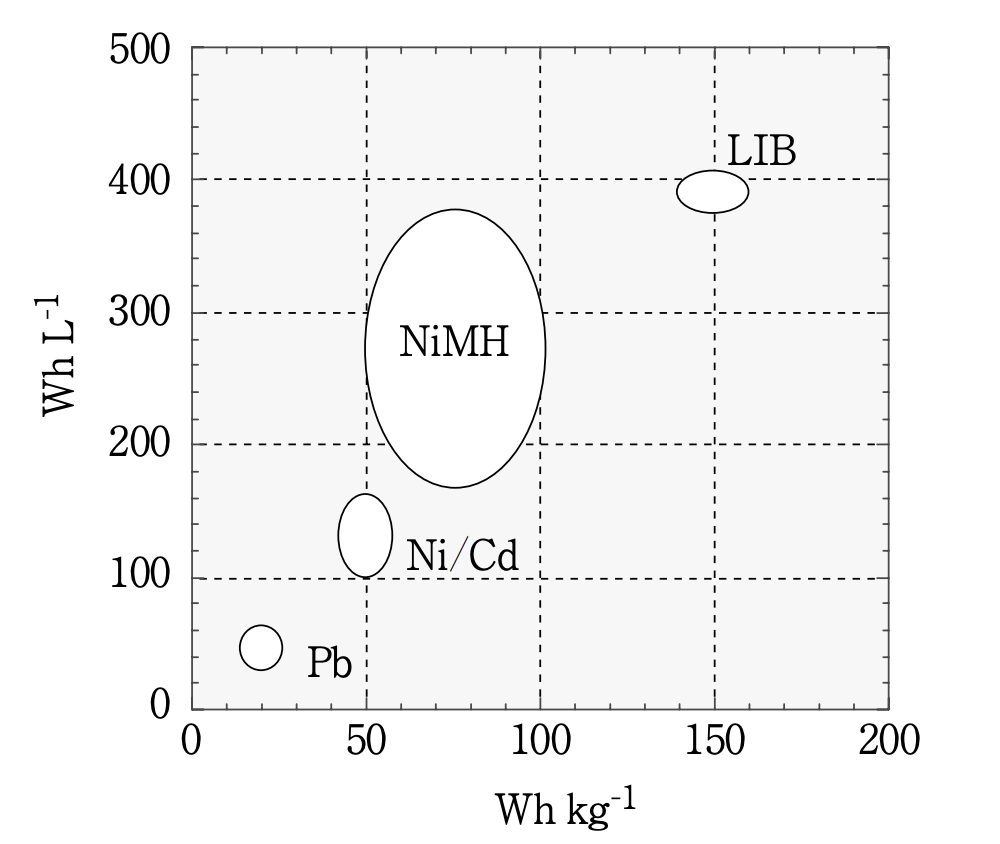
\includegraphics[width=8cm]{src/fig/fig1.png}
\caption{The energy density in different secondary batteries}
\end{figure}
However, for the practical applications in EVs where a large number of LiBs are packed together and used for high power output. The optimal performance LiBs is expected to be: (1)high specific capacity; (2)high durability and safe ; (3)long cycle life; (4)lightweight.

Since the current anode and cathode materials have almost reached their ideal capacities, the development of next-generation LiBs is expected through the research on new materials.

Generally, a lithium-ion battery consists of an anode, cathode, current collector, electrolyte, and separator. The electrodes repeat charging and discharging, converts chemical energy to electric energy, or vice versa, by redox reactions. Charging causes the Lithium ions within the crystal structure of the cathode material to be extracted and inserted into the anode material. During discharging, Lithium ions stored in the anode move to the cathode. The electrons travel through an external circuit thus forming a closed circuit. Both anodes and cathodes allow Li+ insertion and extraction without major changes to the host structure. A separator that allows ions to shuttle through, which is necessary to prevent from making direct contact between the electrodes.
\begin{figure}[h]
\centering
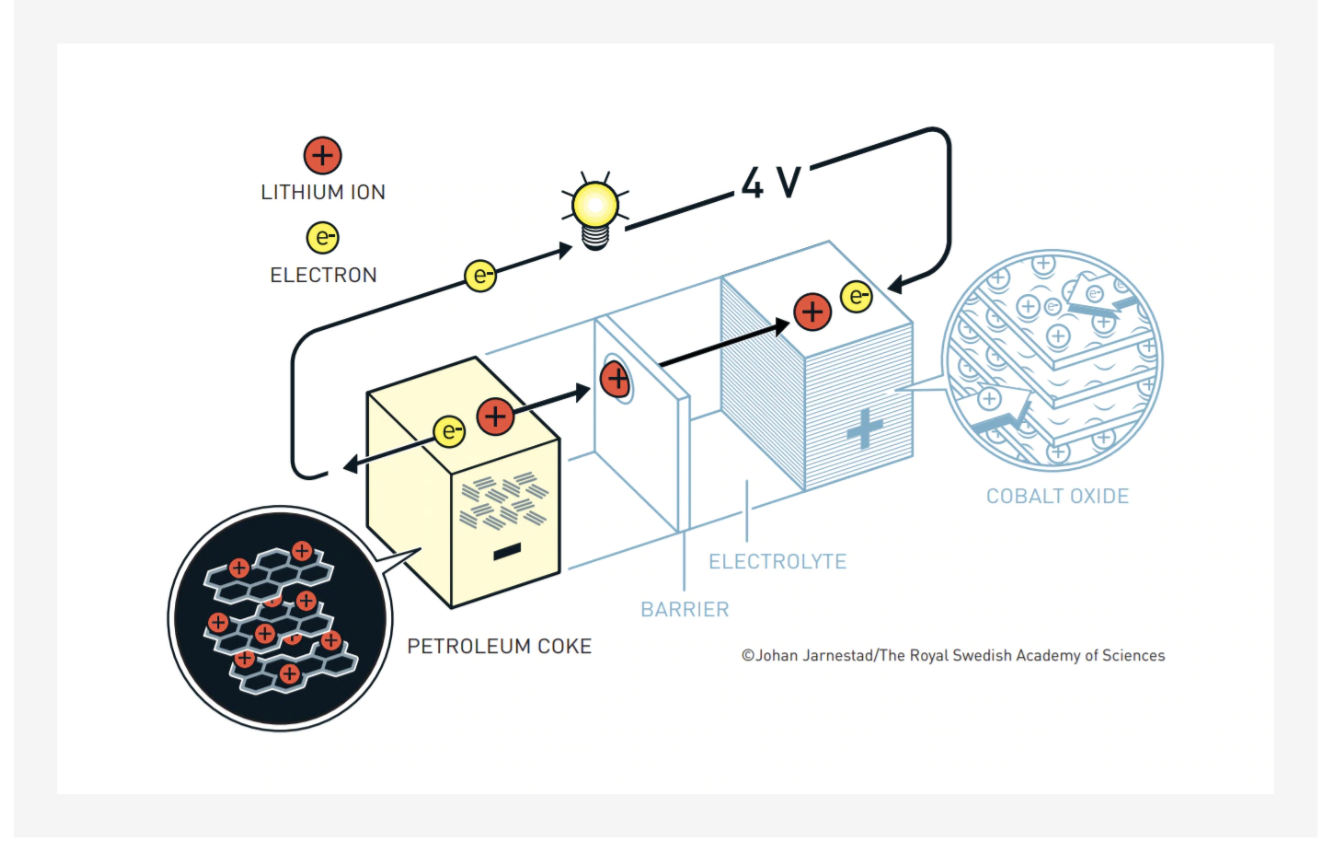
\includegraphics[width=8cm]{src/fig/fig2.png}
\caption{Schematic illusion of a LIB\textsuperscript{[2]}}
\end{figure}
The charging and discharging reactions of this battery can be expressed as follows:
$$L i_{1-x} C o O_{2}+x L i^{+}+x e^{-} \Leftrightarrow L i C o O_{2}$$
$$L i_{x} C_{6} \Leftrightarrow x L i^{+}+x e^{-}+C_{6}$$
\subsubsection{Cathode:}
The cathode, also called the positive electrode, functions within the battery as an oxidant during discharge. Cobalt-based cathodes ($\mathrm{LiCoO_{2}}$) are the most common cathode used in LiB due to high equilibrium potential. $\mathrm{LiCoO_{2}}$ has lithium and cobalt laminated between oxygen layers, and the charge/discharge reaction is repeated by intercalation–deintercalation of large amounts of lithium ions. In recent years, significant researchs have focused on other layered positive electrode materials, in which the Co or Ni of $\mathrm{LiCoO_{2}}$ and $\mathrm{LiNiO_{2}}$ are replaced by other transition metals. 
\subsubsection{Anode:}
The anode, as the negative electrode active material, is a reducing agent with a lower potential during discharging. So anode materials should have a low potential corresponding to a standard electrode and provide a high cell voltage with the cathode. Graphite-based anodes are the dominant materials in the anode market for their low voltage, excellent performance, and most of all, low cost. However, nowadays, the low capacity of graphite no longer meet the energy needs. Materials like Si and Sn have with higher capacity have attracted scientists attention.
\subsubsection{Electolyte:}
Within a battery, the electrolyte is the most important component after the positive and negative electrodes. For a practical battery, the choice of electrolyte often has a large effect on the characteristics of the battery, such as the operating voltage and the energy density. A wide variation of electrolytes has been used in solid, molten or liquid form.
The following gives some of the general properties that an electrolyte for a practical battery should have:
\begin{itemize}
\item High ion conductivity
\item Wide potential window
\item Thermal and chemical stability
\item No or low toxicity
\end{itemize}
The major discovery of electrolyte focus the selection of binary solvent mixtures such as ethylene carbonate (EC) and either dimethyl carbonate (DMC), ethyl methyl carbonate (EMC) or diethyl carbonate (DEC), and the Li salt, lithium hexafluorophosphate ($\mathrm{LiPF_{6}}$), as the basic standard electrolyte solutions for Li-ion batteries.
\subsubsection{Separator:}
Separators are nonactive materials that do not participate in electrochemical reactions. They provide a pathway for ion transport that is essential for battery operation and separate physical contact between the anode and the cathode. Typically, separators are micro porous polymer films with a porosity of 30–50\% and the thickness ranging from manometers to micrometers. The most commonly used separators are polyolefins such as polyethylene(PE) and polypropylene (PP), and these materials have various advantages including outstanding mechanical strength, chemical stability, and low cost. If the temperature rises during internal short circuits, the melted separator blocks pores and restricts ion movement, thus improving battery safety by delaying thermal reactions.
\subsubsection{Cell container:}
The components of LIB should  be appropriately packaged in a container. To satisfy the requirement of lightweight and robust, metal containers are often used. In addition, thermal exchange properties and crush/crash worthiness are also important factors for a long-term service of battery. Rubber gaskets used in a container act as seals to prevent electrolyte from leaking out and moisture in the air from infiltrating the battery.
\subsection{Next-generation Si-based anodes\textsuperscript{[1]}}
Graphite is the most commonly employed material in the LIB anode due to its low cost and good stability. Graphite is composed of hexagonally bonded sheets of $\mathrm{sp^{2}}$ hybridized carbon that bounds with sub-sequent sheets through van der Waals force. Intercalation/deintercalation process (the insertion/withdrawal of Li+ ions) takes place in between the planes of the graphite. The formation of intercalation compound $\mathrm{LiC_{6}}$ provides a theoretical specific capacity limit of 372 mAh/g.
To satisfy the need for large-scale portable energy sources, alloy-type anodes have been intensively explored due to their high capacity. From a material’s point of view, Silicon(Si) has been receiving tremendous attention in recent years. First, the discharging potential of Si, about 0.2 V with respect to Li/Li+ , is lower than most of other alloy-type or metal oxide anodes. Second, Silicon has the highest theoretical capacity of 4200 mAh/g upon full lithiation with the formation of $\mathrm{Li_{22}Si_{5}}$, which is more than 10 times that of commercial graphite. Third, there is a high abundance of Si element in the earth crust and the cost to obtain both single-crystalline and polycrystalline Si has dropped to an acceptive range. Also, there are other merits of Si, such as good environmental compatibility, low toxicity, and relatively stable chemical compatibility, low toxicity, and relatively stable chemical property, and all these make Si a very promising candidate for next-generation anode.
\begin{figure}[h]
\centering
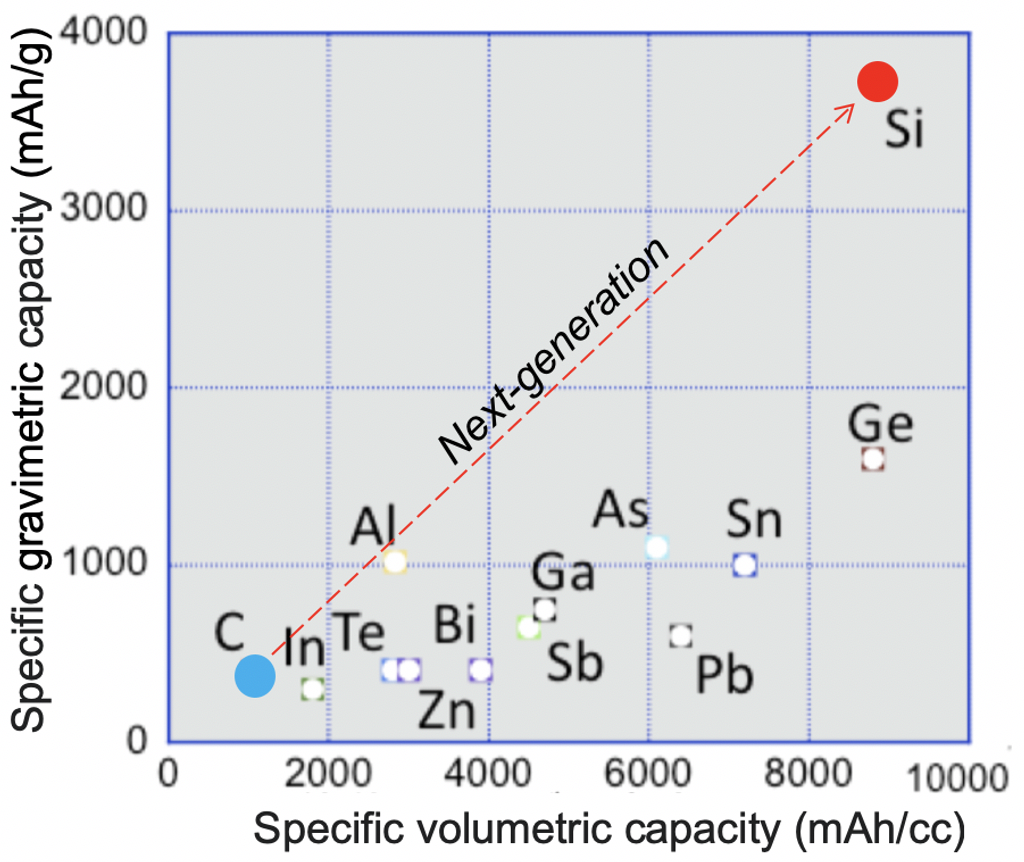
\includegraphics[width=8cm]{src/fig/fig3.png}
\caption{The specific capacity of elements}
\end{figure}
However, the practical implementation of Si anodes is still blocked due to three major problems. First, silicon has poor electronic conductivity. Second, Si anode usually suffers from large volume change (>300\%) and mechanical fracture within 10 cycles. Finally, the solid electrolyte interphase (SEI) breaks as the nanostructure shrinks during delithiation. This results in the exposure of the fresh silicon surface to the electrolyte and the reformation of the SEI, resulting in the SEI growing thicker with each charge/discharge cycle. These side effects lead to poor cycle-life, drastic irreversible capacity loss and low coulombic efficiency of Si anode. other high capacity materials such as tin (Sn), germanium (Ge), and antimony (Sb) have the same volume change issue. 

To address these issues, several strategies have been developed to accommodate the huge volumetric changes. Tremendous exploration on materials has been made.
\begin{figure}[H]
\centering
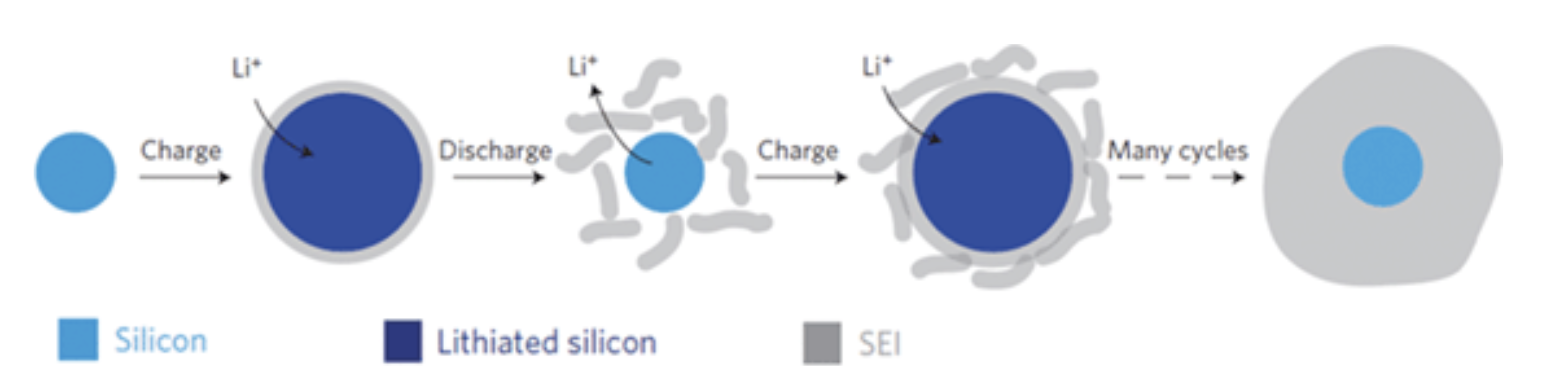
\includegraphics[width=10cm]{src/fig/fig4.png}
\caption{Schematic of SEI formation on silicon surfaces\textsuperscript{[3]}}
\end{figure}
As one effective strategy to suppress the volume change, Silicon is produced in dimensions of tens of nanometers. According to the research of J. Graetz\textsuperscript{[4]}, nanocrystalline silicon exhibited specific capacities of ~ 1100 mAh/g with a 50\% capacity retention after 50 cycles. The amorphous thin-film electrodes exhibited initial capacities of 3500 mAh/g with a stable capacity of ~2000 mAh/g over 50 cycles. The capacity and cycle performance were greatly enhanced in nano-size Si structure, compared with bulk Si.
\begin{figure}[H]
\centering
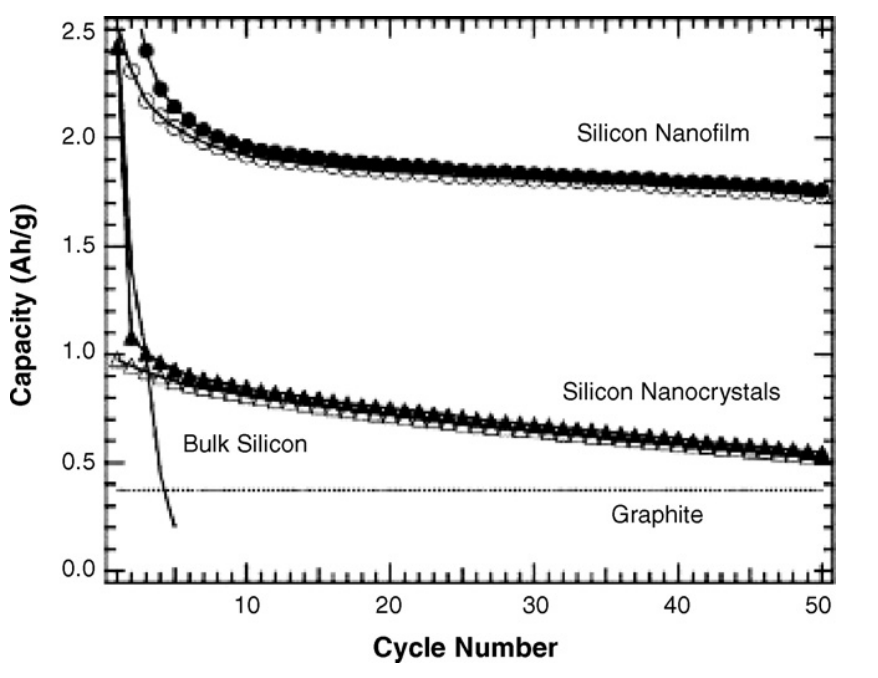
\includegraphics[width=8cm]{src/fig/fig5.png}
\caption{Specific capacity vs. cycle number for nano-crystalline Si, nano-amorphous Si thin film anodes, graphite and bulk-silicon anodes\textsuperscript{[4]}}
\end{figure}
\begin{figure}[H]
\centering
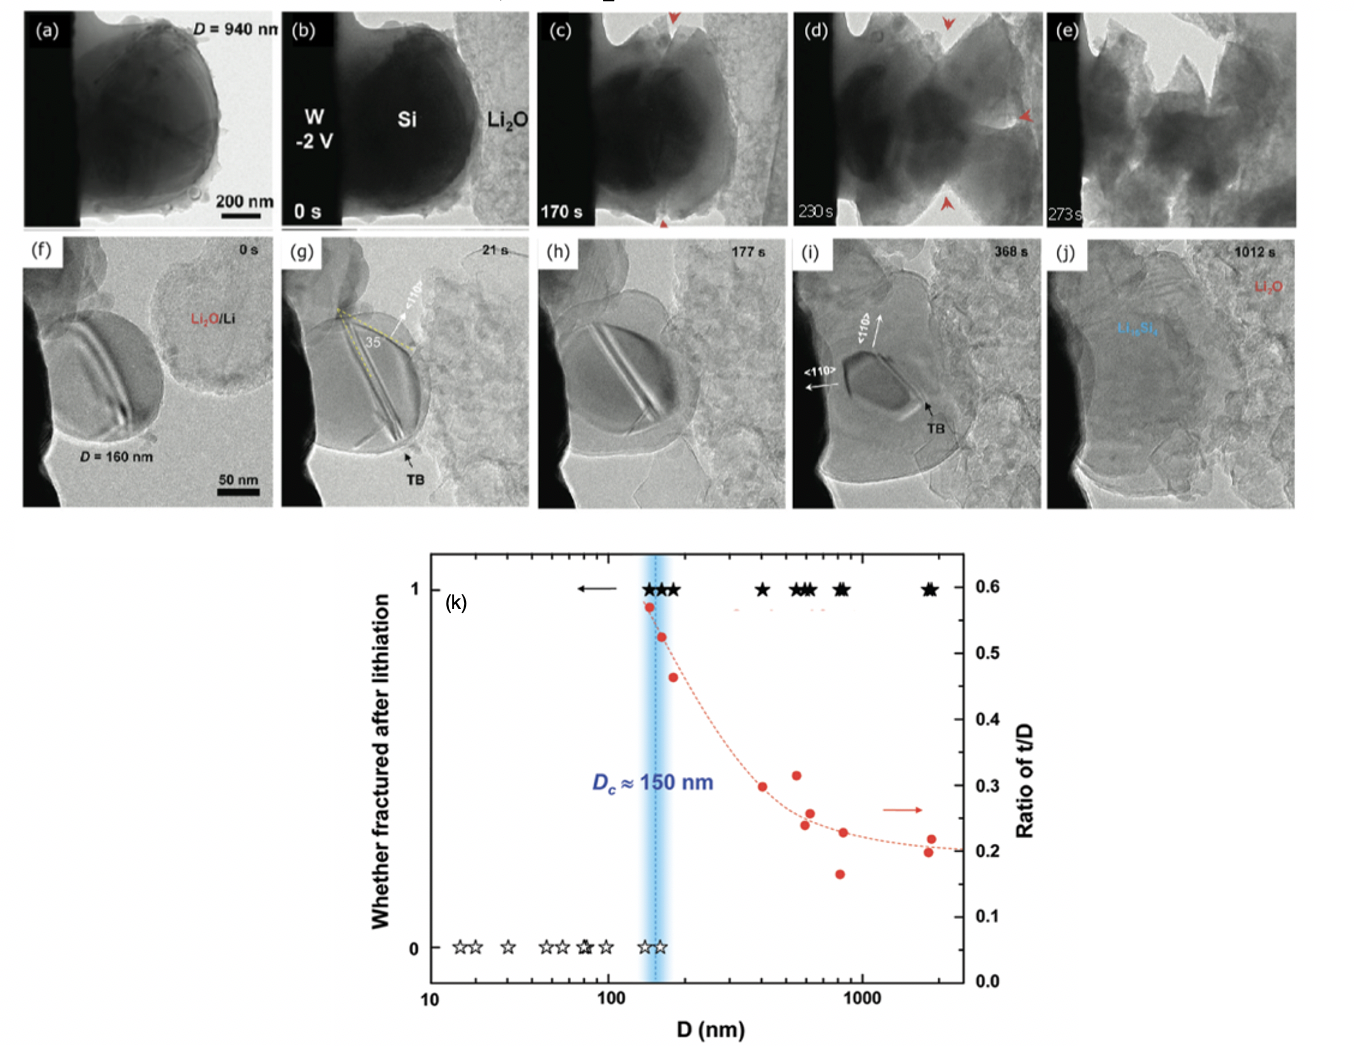
\includegraphics[width=14cm]{src/fig/fig6.png}
\caption{The lithiation of SiNP with diameter (a)--(e) D=940 nm, (f)--(j) D=160 nm, (k) The relationship between Si particle size and fracture.\textsuperscript{[5]}}
\end{figure}
The in situ TEM observations by Liu\textsuperscript{[5]} confirmed that the lithiated Si structure breaks during Li alloying reaction process in one minute. As shown in figure 1.6, the pristine SiNP (D=940 nm) multiple cracked at different locations eventually fracture occurred. In contrast, for a smaller SiNP (D=160 nm), no cracks was observed till Si attained full lithiated state $\mathrm{Li_{15}S_{4}}$. This observation was in good agreement with critical size $\mathrm{D_{C}}$ of about 150 nm, which was from statistics result. 
In addition, figure 1.6(i) shows the expansion along <110> directions is 170\%, while along <111> directions the swelling is less than 20\%. This result indicates that lithiation-induced swelling is preferably along the <110> directions in Si nanowires, which is consistent with the anisotropic expansion of the SiNP.

Despite the advantages of nanostructured Si anodes, nanosized particles also have disadvantages such as large surface area, high manufacturing costs, and difficulty of handling. Even so, nanostructured silicon is regarded as one of the most promising methods to overcome the challenges of silicon anodes for next-generation lithium-ion batteries.
%\vspace{-10em}
\subsection{Si@carbon nanocomposite}%1.1.3
%\vspace{-7em}
Another approach to overcome the volume change during cycling is to form Si-carbon composites. The carbon material is usually used ad a buffer matrix that prevents the significant volumetric change of Si, maintaining the structural integrity of the electrode, and enhancing stability by reducing silicon aggregation or electrochemical sintering. Also, due to the limited electrical conductivity of Silicon, carbon additives can improve battery performance. There are several structure designs of Si-carbon composite.
%\vspace{-14em}
\subsubsection{(i)core-shell/yolk-shell\textsuperscript{[6]} }
%\vspace{-7em}
\begin{figure}[H]
\centering
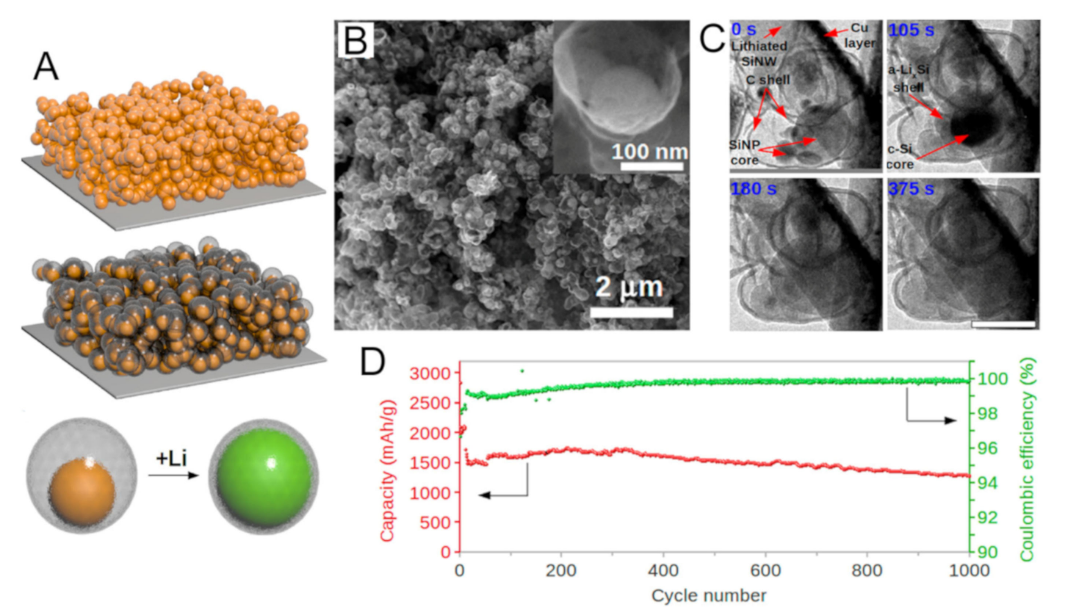
\includegraphics[width=14cm]{src/fig/fig7.png}
\caption{Si@C yolk–shell nanostructure. (A) Comparison of a conventional slurry coated SiNP and Si@C yolk–shell nanostructure. (B) SEM image of Si@C yolk–shell nanostructure. (C) Serial in situ TEM images showing the expansion of the Si yolk part. The scale bar is 200 nm. (D) Delithiation capacity and Coulomb efficiency of the first 1000 galvanostatic cycles between 0.01-1 V at 1 C rate.\textsuperscript{[6]} }
\end{figure}
Core-shell/yolk-shell nanostructures indicate a class of hybrid materials consisting of a hollow shell encircling movable cores with the void. The additional space between the core and the shell, usually carbon or silicon oxide, can buffer the volume expansion significantly. The outer shell remains unchanged during cycling, and thereby helps the formation of a stable SEI layer, thus electronic conductivity is promoted.
Cui and co-workers have made pioneer work in this field[4]. The completely sealed Si@C yolk–shell structure was monitored with in-situ TEM to demonstrate that the Si@C yolk–shell provides excellent electrochemical cycling performance to alleviate the severe volume change of Si during lithiation/delithiation (Figure 1-7C). Pristine Si nanoparticles (0s) are visible within the outer Carbon shell. The volume expansion of Si nanoparticles is seen in 105s to produce the partially lithiated LixSi shell/crystalline Si core in the carbon shell. Full lithiation increases the size of Si particles up to ~300 nm. Furthermore, the thickness of carbon shell increases from 5 to ~20 nm after lithiation implying that the carbon coating is also lithiated and creates a thin layer of ionic liquid electrolyte at the surface. Figure 1-7D shows the reversible capacity of Si@C yolk–shell electrode reached 2833 mAh/g for the initial cycle at C/10 and stabilized at ~1500 mAh/g at 1 C. No capacity retention was observed in the first 300 cycles and 74\% of the capacity was achieved after 1000 cycles. 
\subsubsection{(ii)Si-graphene/Si-carbon coating\textsuperscript{[7]}}
Graphene has also been used in Si anodes to buffer the volume changes and improve electronic conductivities due to its superior electrical conductivity, high surface area, excellent chemical stability, and strong mechanical strength. Pan[5] prepared silicon@carbon@graphene micro-sized composite (Si@C@RGO) using an industrially scalable spray drying approach and a subsequent calcination process. As fig.1-9 shows, The obtained Si@C@RGO anode exhibits a high initial reversible specific capacity of 1599 mAh/g at a current density of 100 mA/g. Moreover, the Si@C@RGO anode shows a high reversible specific capacity of 951 mAh/g  even at a high current density of 2000 mA/g . The excellent cycling stability and superior rate capability are attributed to the unique structural design of carbon coating and wrapped by highly conductive graphene. The combination of carbon shells and flexible graphene can effectively enhance the electrical conductivity of the composite and accommodate significant volume changes of silicon during cycling.
\begin{figure}[H]%  强制放图片
\centering
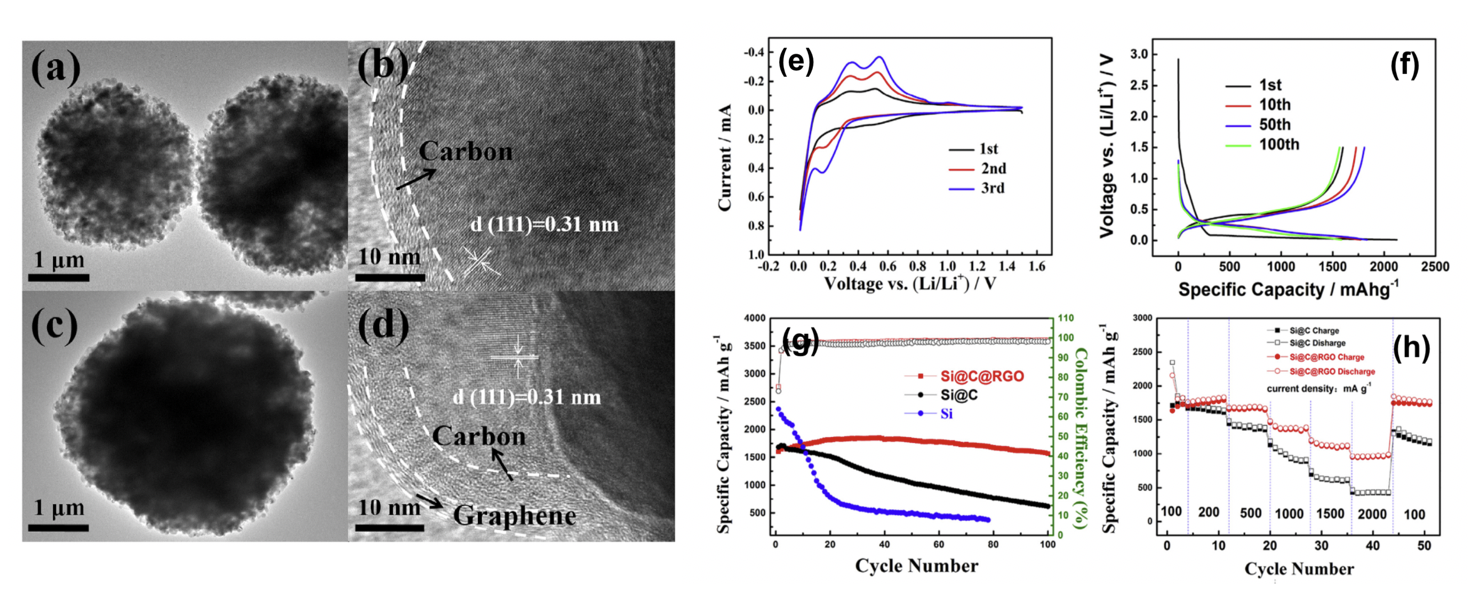
\includegraphics[width=14cm]{src/fig/fig8.png}
\caption{HRTEM images of (a, b) Si@C and (c, d) Si@C@RGO
composite;(e) CV curves of the Si@C@RGO anode at 0.1 mV/s  between 0 and 1.5 V for the first three cycles; (f) Charge/discharge voltage profiles of Si@C@RGO composite for the 1\textsuperscript{st}, 10\textsuperscript{th}, 50\textsuperscript{th}, 100\textsuperscript{th} cycle; (g) Cyclic performance of Si, Si@C and Si@C@RGO composite at a current density of 100 mA/g in the first three cycles and then continued at 200 mA/g thereafter; (h) Rate performance of Si@C and Si@C@RGO composite at various current densities\textsuperscript{[7]}.}
\end{figure}

\subsubsection{(iii)Si-carbon nanotubes(Si@CNF)/Si-carbon nanofibres(Si@CNF) composite\textsuperscript{[8]}}
Recently, CNTs has received considerable attentions as a candidate material for the LIB application. Different from other allotropes of carbon, CNT is a 1D structure with a large aspect ratio(length--to--diameter) in excess of 1,000. CNTs can be regarded as nanoscaled cylinders composed of rolled up graphene sheets around a central hollow core. There are two types of CNTs: single-walled carbon nanotubes (SWCNTs) and multi-walled carbon nanotubes (MWCNTs), and the later consist of two or more graphene layers with van der Waals forces between adjacent layers. However, growing  SWCNTs requires strict growing condition such as high temperature. That is because their small diameters results in high curvature and high strain energy to maintain its crystalline. A perfectly structured CNTs possess amazing mechanical properties such as Young’s modulus, which are favored especially in energy storage field. This is due to the chemical bonding of $sp^{2}$ in CNTs. 

As to application of CNTs in LIB,the incorporation of CNTs as an additive to active materials is an effective strategy to form conductive networks in the electrode at a content much lower than other carbonaceous materials, like carbon black and graphite. Various anode materials with and without CNT additives have been studied, undeniably confirming much enhanced cycle performance of the nanocomposites containing MWCNTs as compared to the neat anode materials.

MARUBAYASHI\textsuperscript{[9]} had employed the thin-layered graphite (TLG) and the artificial graphite (AG) as conductive additives for improving the conductivity of the $\mathrm{LiCoO_{2}}$ (LCO) cathode, in either case the small amount of MWCNT improved the capacity retention ratio. Xue et al.\textsuperscript{[10]} had produced carbon coated Si nanoparticles then dispersed them in a CNT network. Electrochemical test result indicates the Si@C-CNTs show capacity retention of 70\% after 40 cycles, which is much better than the Si@C nanoparticles without CNTs. The tangled CNT network is believed to  better accommodate of the strains arising from Li ion insertion/extraction to maintain the integrity of electrodes, stabilize the electric conductive network for active Si, and eventually lead to better cycling performance. In addition, it is reported that The CNTs can facilitate rapid Li ion transport through the large electrode–electrolyte contact area and work as fast electron transport pathways.[6] 
\begin{figure}[H]
%\centering
\begin{minipage}[t]{0.5\textwidth}
 \centering
 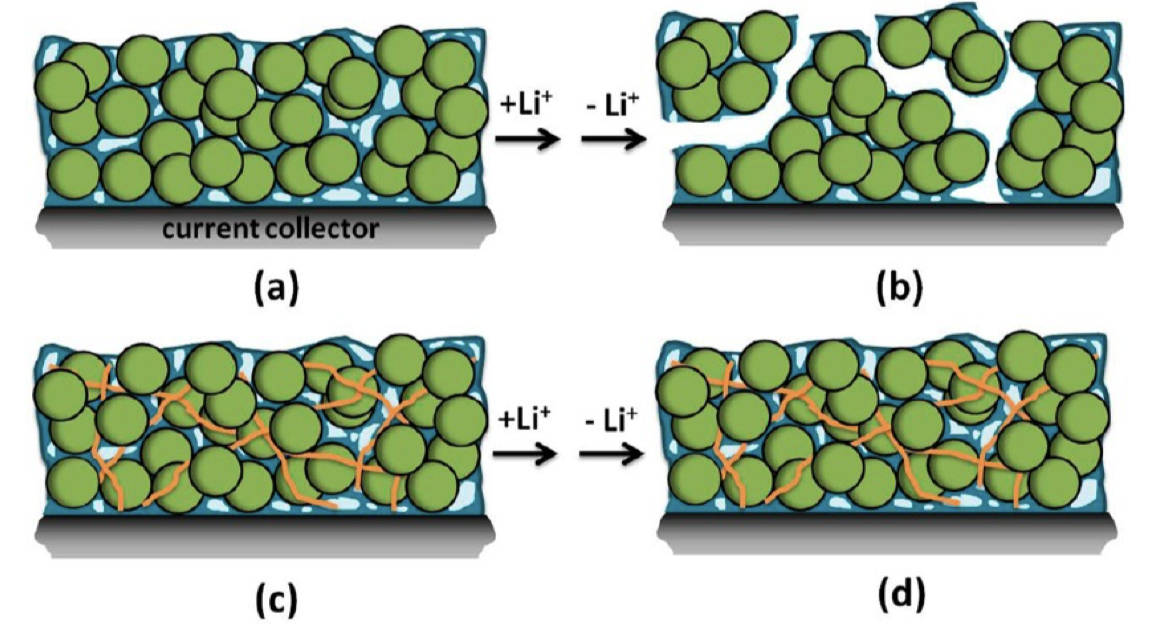
\includegraphics[scale=0.35]{src/fig/fig9.png}
 \caption{Schematic of a Si@C with binder (a) before and (b) after cycling, and Si@C--CNTs with binder (c) before and (d) after cycling\textsuperscript{[10]}.}
 \end{minipage}
%\hfill
\begin{minipage}[t]{0.5\textwidth}
%\centering
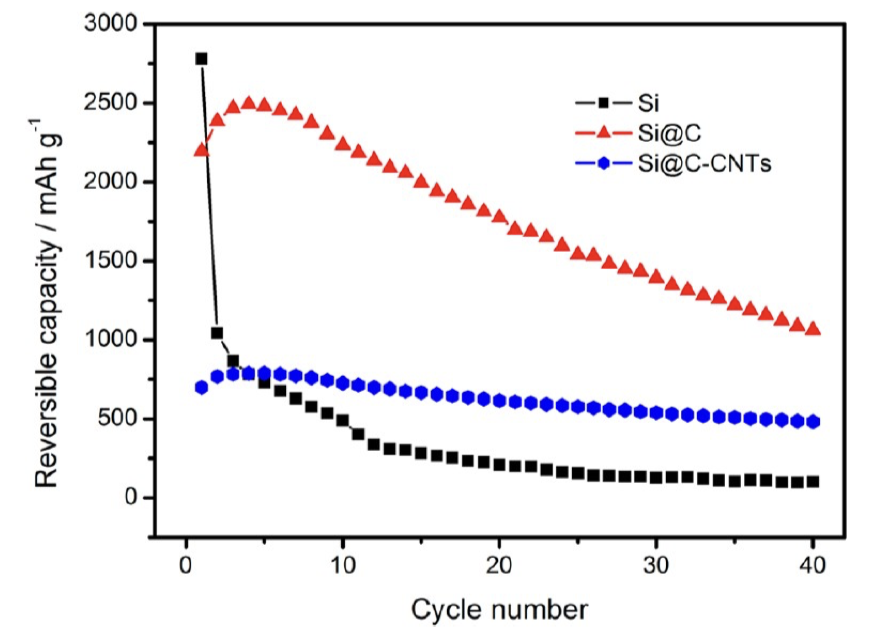
\includegraphics[width=7cm]{src/fig/fig10.png}
\caption{Cycling performance of Si, Si@C, and Si@C-CNTs at 100 mA\/g and within a voltage window of 0.02-2.0 V\textsuperscript{[10]}.}
\end{minipage}
\end{figure}

The term  ‘tube’  refers to those sheets rolled up into concentric cylinders. If the stacked-cone structures exhibit only small $\theta$  values and are not cylinders but are mostly hollow, the can be called multi-walled carbon nanofibres (MWCNFs). Also, CNFs are much bigger,more disordered, less oriented, with a large number of  defects.  Hence the mechanical properties of CNFs are as  outstanding as of CNTs, especially the single-walled ones , but still high enough to be used in LIB. [Effect of CVD carbon coatings on Si@CNF composite as anode for lithium-ion batteries]). On the other hand, defective CNTs were reported to be more effective for the adsorption and diffusion of lithium ions. 

\section{Plasma-spray PVD}
\subsection{Feature of plasma\textsuperscript{[11]}}
Plasma is the fourth state alongside solids, liquids, and gases. It is a special kind of ionized gas and in general consists of positively charged ions , electrons, and neutrals (atoms, molecules, radicals). A typical example is the sun, whose interior temperatures exceed 107K. The plasma stays quasi-neutral and its properties are dominated by electric and/or magnetic forces .
There are two types of plasma, non-thermal plasma and thermal plasma. Non-thermal plasma is usually generated by glow discharge at low pressure, and mostly contains unionized neutral gas particles. In a non-thermal plasma, only the electron temperature($T_{e}$) is high and other species like heavy particles and ions stay at relatively temperature. Therefore, such plasma is called non-equilibrium plasma or low temperature plasma as well. On the other hand, thermal plasma is generated by arc discharge at higher pressure range, which possess a higher ionization level. The electron temperature Te, ion temperature Ti, and neutral temperature Tn are almost equal (5,000 K -- 20,000 K).

\begin{figure}[h]
\centering
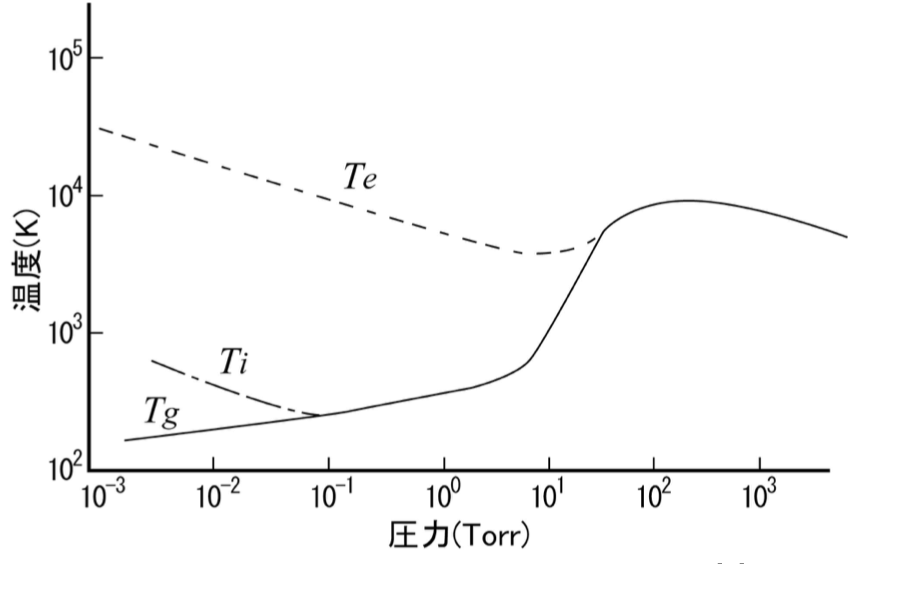
\includegraphics[width=8cm]{src/fig/fig11.png}
\caption{The temperature in a plasma as a function of pressure\textsuperscript{[14]}}
\end{figure}
Today, plasma technology is applied to the field of deposition of coatings and films. One typical method is Plasma spray physical vapor deposition (PS-PVD). PS-PVD is recognized as a high throughput process for production of nanoparticles and nonstructural coatings by completely evaporation, quenching and condensation on a relatively cooler substrate. Compared to other surface coating technologies, the major advantages of PS-PVD are as follows:
\begin{itemize}
  \item The thermal plasma can heat up feed stock materials quickly and effectively, for its high temperature and active species. Therefore, the deposition rate is high, enables PS-PVD technology to meet the industrial requirements.
  \item The substrate can stay at a relatively low temperature, namely the quality of the substrate itself can be maintained.
  \item By selecting different gases to generate plasma, it is possible to create a wide range of conditions, such as oxidizing atmosphere ($\mathrm{O_{2}}$), inert atmosphere (Ar), or reducing atmosphere ($\mathrm{H_{2}}$), etc.
\end{itemize}

\subsection{Types of Plasma spray\textsuperscript{[15]}}
Plasma spraying systems can be categorized into three types based on the plasma jet generation method.
\begin{figure}[H]
\centering
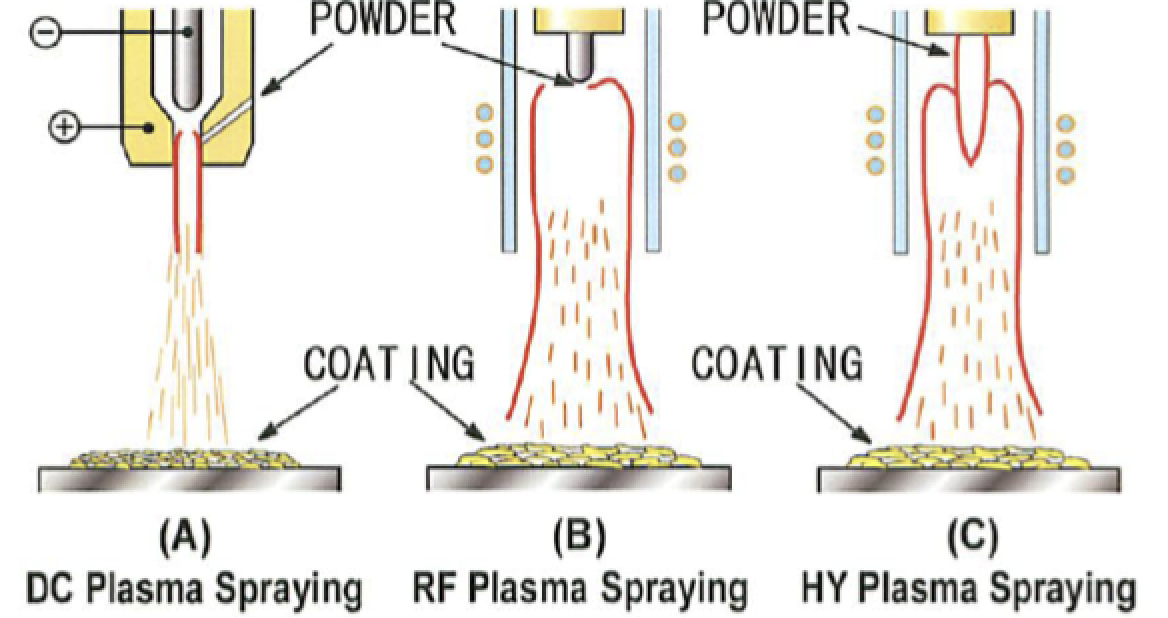
\includegraphics[width=10cm]{src/fig/fig12.png}
\caption{Plasma generated by (a)direct current; (b)radio frequency; (c)hybrid torch\textsuperscript{[15]}}
\end{figure}
\subsubsection{(a)	Direct-current (DC)}
A high--intensity arc is generated by a direct current and operated between a stick-type cathode and a nozzle-shaped anode. This Cupper anode is usually water-cooled, establishing a sharp temperature drop in plasma, in order to confine the arc expansion and guarantee an energy constriction. This effect is called “thermal pinch”. The figure below shows the temperature and flow velocity distribution of a typical Ar-$\mathrm{H_{2}}$ DC plasma. It is generated at an arc voltage of 52V, an arc current of 500 A. The flow rate of Ar is 44 L/min and of $\mathrm{H_{2}}$ is 7 L/min. There is a sharp temperature and velocity drop along with the axial directions. Using the enthal--peeve method, the temperature gradient is found to be 250 K/mm and the velocity gradient is about 10 m/s/mm. Ideally, the powder should be fed to the center of the plasma for sufficiently evaporation. However, but in DC plasma, the powder is injected in the direction that is perpendicular or angled(45°) to the plasma jet. The plasma gas is highly viscous and flows at high speed, the lightweight particles and heavy particles are carried at different orbits, result in an nonuniform coating.
\begin{figure}[H]
\centering
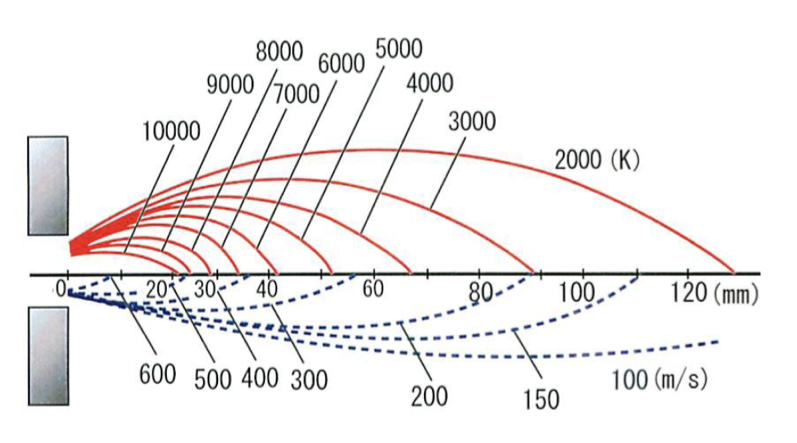
\includegraphics[width=10cm]{src/fig/fig13.png}
\caption{The temperature and velocity axial distribution in DC plasma jet\textsuperscript{[13]}.}
\end{figure}

\subsubsection{(b) Radio-frequency (RF)}
There are several types of plasma that use radio frequencies, but here the most used one, inductively coupled plasma (ICP), is addressed. In ICP, The current produced by electromagnetic induction, namely, by time-varying magnetic fields. This current flows in a cylindrical coil that surrounds the plasma bulk. The frequency for generating plasma is determined by the diameter, gas type, and power. The benefits of using ICP are as follows:
\begin{itemize}
  \item Due to the absence of electrodes in an ICP, the axial injection of the feed stock is realised.
  \item The RF discharge permits particles a relatively long in-flight heating time and low velocity(20--30 m/s), which is about an order of magnitude lower than that of DC plasma. As a result, the residence time of substances in the plasma is about 10 ms, and the particles can be melted uniformly and sufficiently.
  \item It is possible to generate plasma that cannot be obtained by other methods such as $\mathrm{O_{2},Cl_{2}, and  F_{2}}$, and there is no contamination of impurities by the electrode material.
  \item A large volume plasma with a diameter of several centimeters can be easily obtained. This is equivalent to 10 times that of a DC plasma.
\end{itemize}
Nevertheless, there are still some cons of ICP. Since the particle velocity is slow, for some materials with high melting point, it's difficult to form a dense film because the droplets already condense before arriving to the substrate. In addition, Since ICP is an electrode--less discharge, the eddy current generated at the time of injecting feed stock is inevitable and cause disturbance to the stability of plasma.

\subsubsection{(c) RF-DC hybrid plasma}
A hybrid plasma is a developed method that combines DC and RF discharge. In hybrid plasma, the DC arc jet is superimposed on the RF plasma centrally, eliminate the possibility of the eddy current generation. In RF, the flow velocity could hardly be controlled, but in hybrid plasma, the input powder rate can be controlled by changing the input of DC plasma, and the appropriate in-flight heating time. Therefore, even for in high melting point materials, the time for staying in the droplet state can be extended till arriving at the substrate, thus a dense film is formed. In hybrid plasma, the temperature distribution is more uniform than that in RF plasma, as shows in fig 1.14.
\begin{figure}[h]
\centering
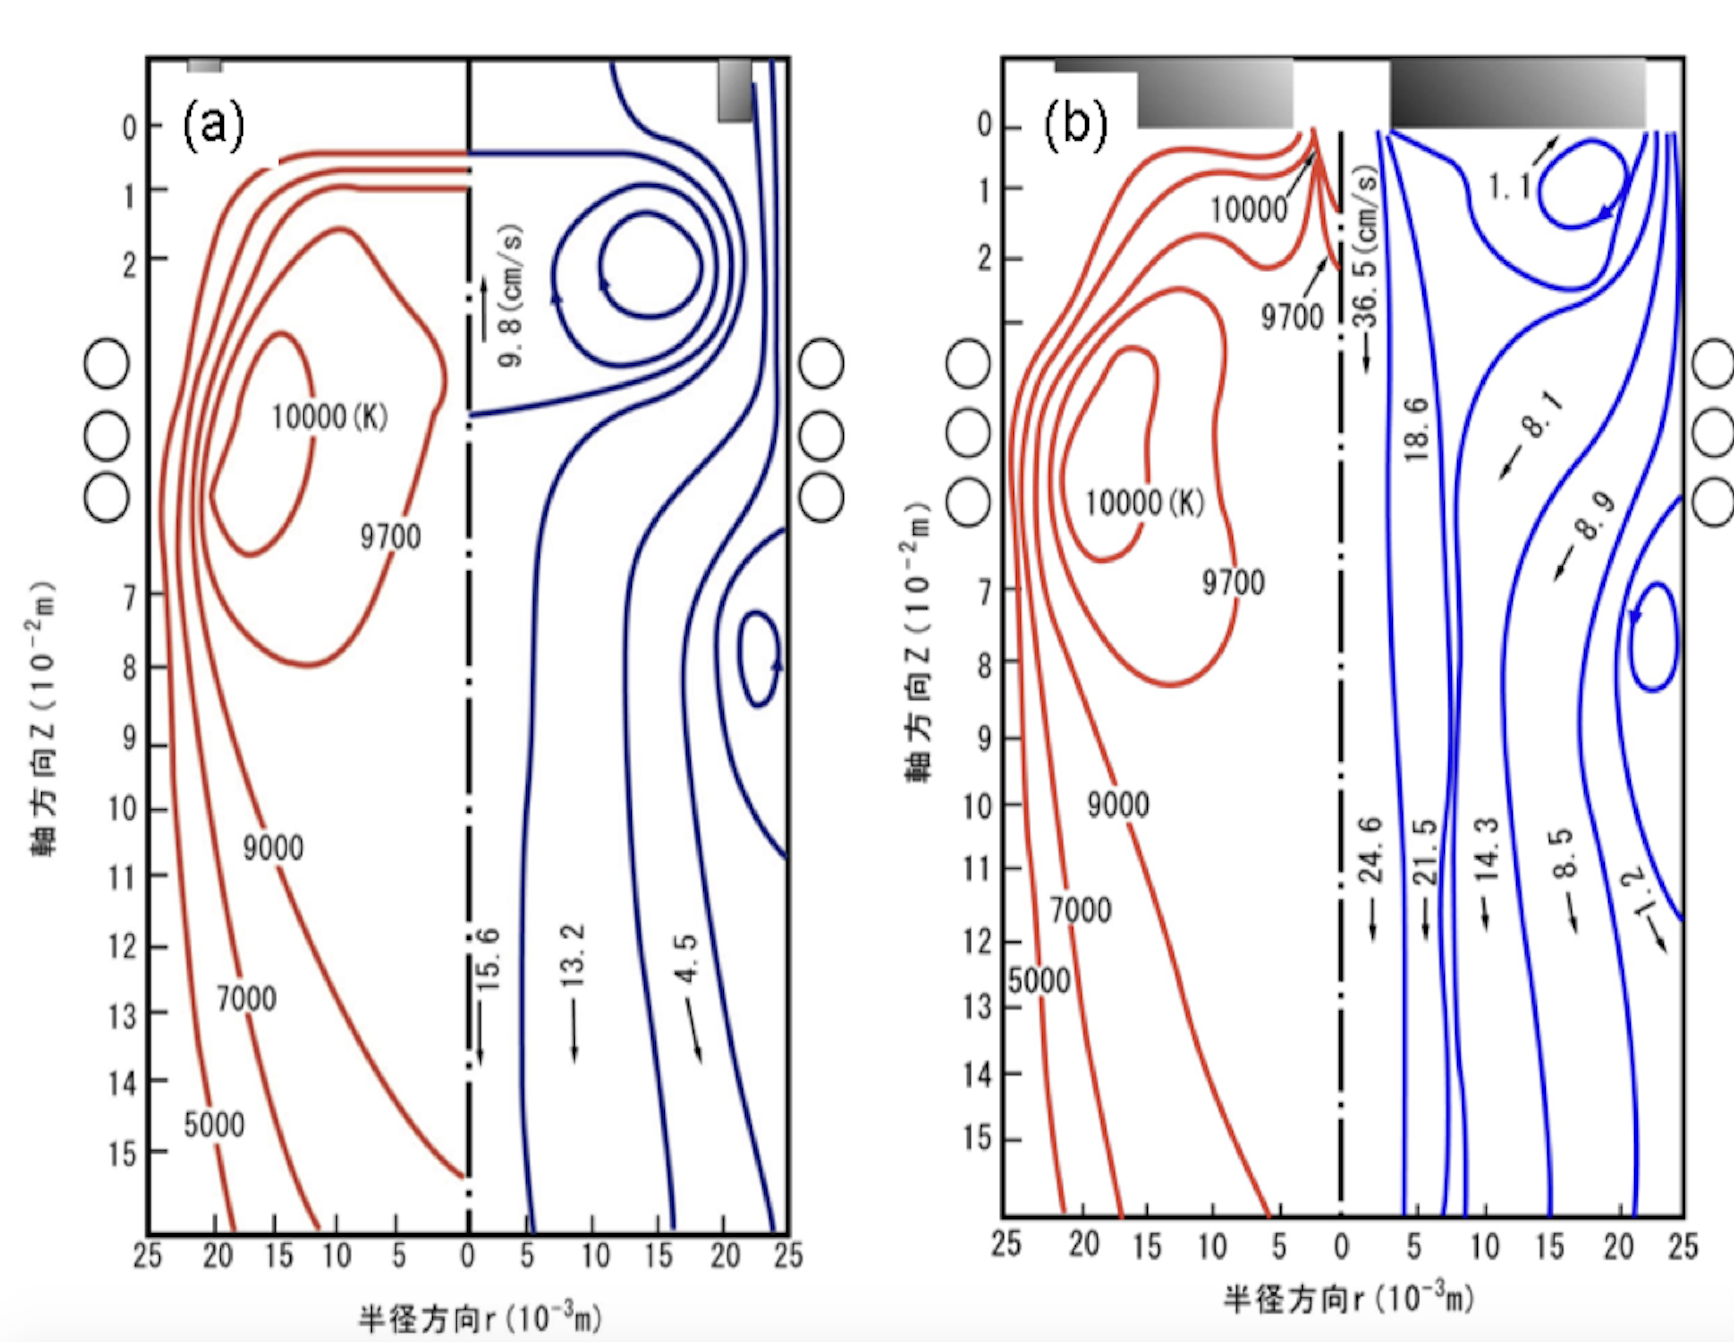
\includegraphics[width=8cm]{src/fig/fig14.png}
\caption{The temperature and velocity distribution in (a) RF plasma (b)Hybrid plasma\textsuperscript{[16]}}
\end{figure}
%没有别的介绍了吗? 我怎么知道你要用PS-PVD去做纳米粒子???
\section{Plasma Enhanced-CVD}
As an advanced method to grow carbon nanotubes, plasma-enhanced CVD features with its low-temperature. In general, carbon nanotubes are produced by basically three methods: laser furnace, the arc, and chemical vapor deposition (CVD). Laser methods are not for large-scale production. The problem with arc material is purification. Thermal CVD and Plasma-enhanced CVD are the popular methods among the market for their salable production, the former method usually requires growth temperature over 700\(^\circ\)C, which is unfavorable for electronic device production. Thus plasma is introduced to lower the temperature of CNT growth. In plasma-enhanced processes, the plasma creates many new and a larger number of reactive species, such as radicals, ions and molecules in excited states, and thus enhances adsorption of carbon-bearing molecules on the catalyst particles providing higher growth rates of the structures as compared with thermal CVD. 

\subsection{Glow discharge\textsuperscript{[16]}}
Typically a glow discharge at reduced pressure is favored for the CNT growth.  As shown in fig.1-15, a glow discharge should be non-thermal, that is, the electron temperature is high but temperature for the heavy species is low.  There are various types of glow discharge plasma. 
\begin{figure}[h]
\centering
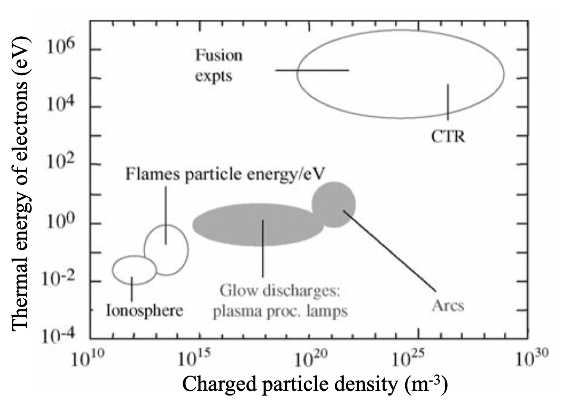
\includegraphics[width=8cm]{src/fig/fig15.png}
\caption{The particle density and electron energy of different plasma\textsuperscript{[16]}.}
\end{figure}
According to Townsend discharge theory, the ignition of plasma needs the electrical breakdown of a gas. The extracted free electrons are accelerated by an electric field, collide with gas molecules, and consequently free additional electrons. Those electrons are in turn accelerated and free additional electrons. The basic version is the direct current (DC) glow discharge, where a continuous potential difference is applied between the fixed cathode and anode, producing a constant current. The breakdown voltage for a specific gas in vacuum is a function of the product of  pressure and distance, which is given by Paschen. 
\begin{figure}[h]
%\centering
\begin{minipage}[t]{0.5\textwidth}
\centering
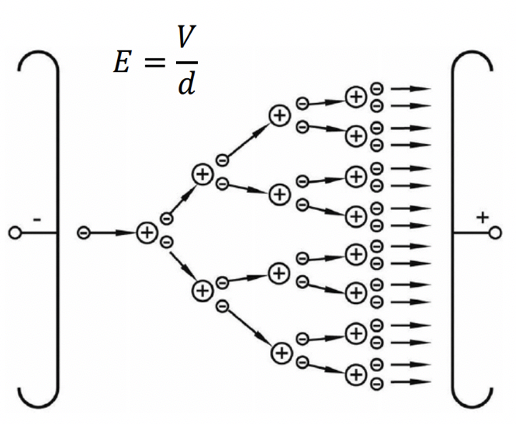
\includegraphics[width=6cm]{src/fig/fig16.png}
\caption{Townsend electron avalanche}
\end{minipage}
\hfill
\begin{minipage}[t]{0.5\textwidth}
%\centering
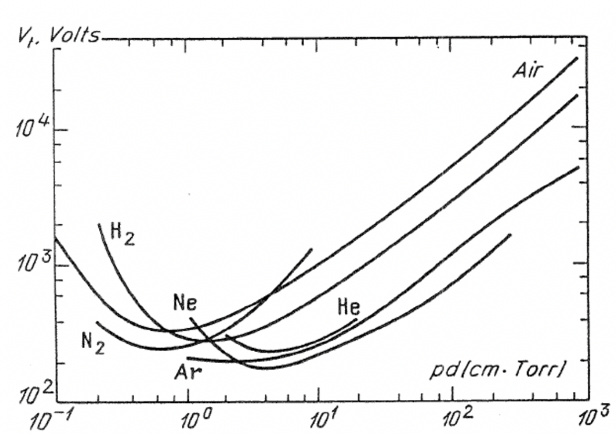
\includegraphics[width=7cm]{src/fig/fig17.png}
\caption{Typical Paschen’s curves\textsuperscript{[17]}}
\end{minipage}
\end{figure}
However, DC glow discharge may give rise to problems when one of the electrodes is non$-$conducting, as due to the constant current, the electrodes will be charged up and leading to burn-out of the glow discharge.  RF breakdown is similar to DC case except that the  high$-$confines electrons by field oscillations$-$multiplication replenishes diffusive losses. Thus the electrons are not as mobile as in DC case.  
\subsection{Low$-$temperature CNT Growth\textsuperscript{[19]}}
Researchers have investigated into growth mechanism of CNT for years. The pioneering work is made by Baker\textsuperscript{[18]}. Researchers have reported various mechanisms. The growth mechanism for most cases proceed as following: (i) the carbonaceous precursors are decomposed onto catalyst and (ii) the atomic carbons diffuse and form a graphitic tubular structure around the particles to form a nucleation seed. (iii) CNT growing from nucleation seed.  It is noteworthy that it’s still unclear whether carbon atoms diffuse on the particle bulk on the particle surface or whether surface and bulk diffusion compete.  

Typical hydrocarbon sources used in plasma-based growth of CNTs include methane, ethylene and acetylene. Since plasma can dissociate the hydrocarbon creating a lot of reactive radicals, the use of pure hydrocarbon feed stock may lead to substantial amorphous carbon deposition, which terminates CNT growth earlier. Therefore, it is desirable to dilute the hydrocarbon with argon, hydrogen or ammonia\textsuperscript{[20]}.
Transition metal catalysts are needed for CNT growth by PECVD, usually Ni, Fe,Co and Mo. Note that the catalyst should be in the form of particles as small as possible in the nanometer range\textsuperscript{[20]}.
\begin{figure}[H]
\centering
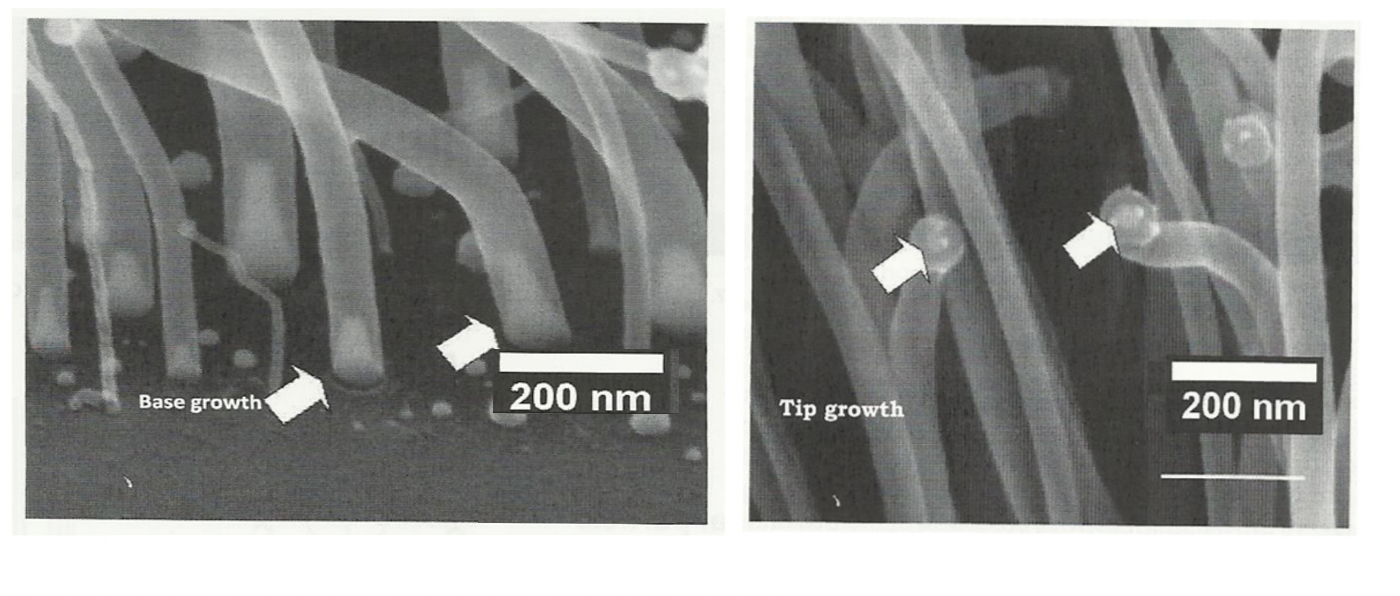
\includegraphics[width=10cm]{src/fig/fig18.png}
\caption{SEM image reveals (a) the base ends of CNTs (b) metallic particles located at the tip of CNTs\textsuperscript{[21]}}
\end{figure}

As fig.1-18 shows, there are two principal morphology of CNT.  The metal catalyst if enwrapped in CNT either within the root or  head. The former is called “base growth”, which usually occurs when metallic particle has strong enough interaction with substrate that cannot be easily separated by the graphite layer formed at the interface in between. On the other hand, if metallic particle and substrate are not strongly connected, the particles will detach and move towards the head of growing nanotubes. This labeled as “tip growth”. 

Generally, according to the state of metal catalyst, the mechanisms can be classified into vapor-solid-solid (VSS), vapor-liquid-solid (VLS) mechanism. V refers to the vapor that contains carbon source.  The middle term  refers to the state of metal catalyst, liquid or solid, dependent on the temperature.  The last term means the solid CNT. In VSS model, to keep the metal catalyst in its solid state, typically a low-temperature condition is needed. Especially in our research,  the solid state of metal catalyst (in our case, Nickel) is of great interest, for the purpose of suppressing silicidation since there is no diffusion barrier. 
\begin{figure}[H]
\centering
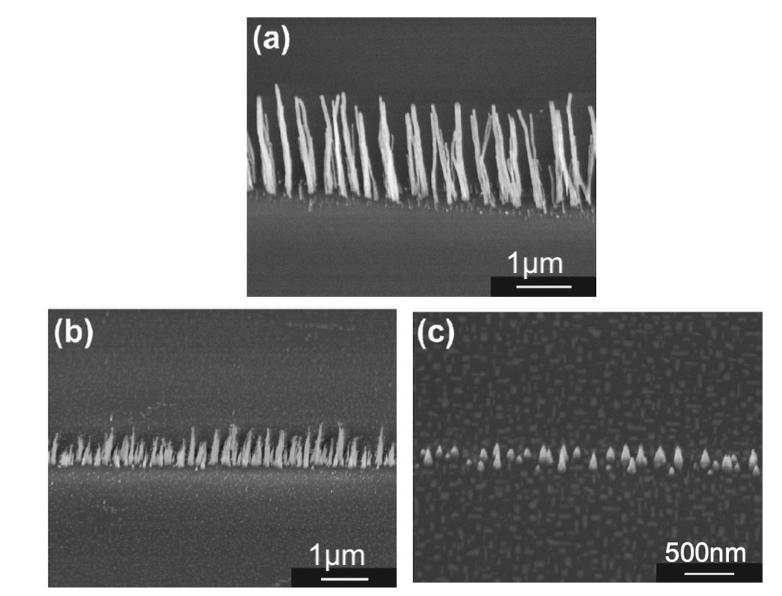
\includegraphics[width=10cm]{src/fig/fig19.png}
\caption{SEM photographs of vertically aligned CNFs grown from e-beam patterned Ni lines at (a)500 \(^\circ\)C; (b)270 \(^\circ\)C; and (c)120 \(^\circ\)C.\textsuperscript{[22]}}
\end{figure}
There have been several reports in the last five years on the growth of MWCNTs by PECVD at low temperature especially under 400\(^\circ\)C and even at room temperature. In these report,s plasma is the essential component.
Hofmann et al.\textsuperscript{[22]}\textsuperscript{[23]} has  successfully grown CNT/CNF at reduced temperature of 120\(^\circ\)C on pre-patterned substrates using a DC PECVD system.  In their work, a DC discharge with the distance between two electrodes was 2 cm, then the plasma was ignited by applying a fixed voltage of 600 V. The $\mathrm{C_{2}H_{2}}$:$\mathrm{NH_{3}}$ ratio was kept constant at 50:200 sccm at a total pressure of 1.5 mbar. A stable discharge current of typically 30 mA was maintained for a fixed deposition time of 30 min.
As shown in figure 1.19,  the higher temperature, the more likely to form tube structure. At 120\(^\circ\)C, the carbon product is more cone$-$shaped. For a conductive addition to anode of LIBs, either CNF or CNT is good enough to promote the battery performance. 
\newpage
\section{The purpose of this research}
In this research, we focus on Silicon:Ni:CNT nanocomposite as anode materials in LiB, for better cycle performance and higher capacity. The target structure is, CNTs with a height of hundred nanometers is grown on Ni nanoparticle, which is directly attached on a larger Si nanoparticle. Ni is expected to be the catalyst for CNT growth.
It's a two step process. First, Si-Ni is prepared using PS-PVD. The nanostructure of processed Si-Ni composite is, Ni directly attached on Si nanoparticles. Based on our previous study, it has been confirmed that both high capacity and high cycle characteristics can be achieved at the same time, compared to bulk Si and nanosized Si without Ni attachment. The reason that select PS-PVD among all nano-technologies, is that, compared to other methods with limited throughput of ~ 1 g / hr at maxium, the PS-PVD process is more industrially oriented for its high throughput at 1kg / hr.
Next, to grow CNT on Si-Ni template. Here we choose low-temperature PECVD to reduce Si-silicidation during CNT growth, otherwise Ni is consumed and terminates the CNT growth at early stage.
Therefore, the purpose of this research is to produce Si:CNT nanocomposite for better battery performance.

\chapter{Experiment}
\section{Plasma Spray-PVD}
\subsection{PS-PVD apparatus}
To produce the Si:Ni nanoparticle, the hybrid plasma with two torch(DC and RF) is used.
\begin{figure}[h]
\centering
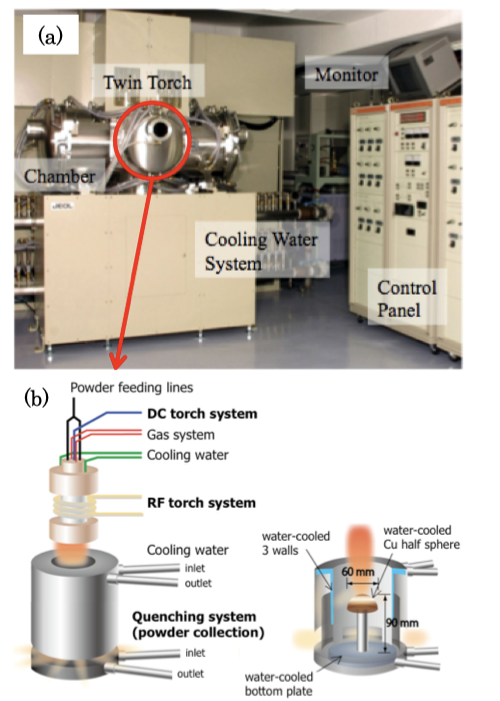
\includegraphics[width=8cm]{src/fig/fig20.png}
\caption{(a)PS-PVD apparatus; (b)illustration of a plasma generator and water-cooling system}
\end{figure}
In the upper part of apparatus, there are two DC torches available for plasma spray process, and here only one torch is used for our research. The maximum DC power is 15 kW and maximum RF power is 150 kW. The chamber is evacuated by a PID pressure controller with a 1200 L/s mechanical booster pump and two 2500 L/s water seal pumps. The pressure can be reduced up to 1 Pa. The detailed condition is described in table 2.1.\\
\begin{figure}[h]
\centering
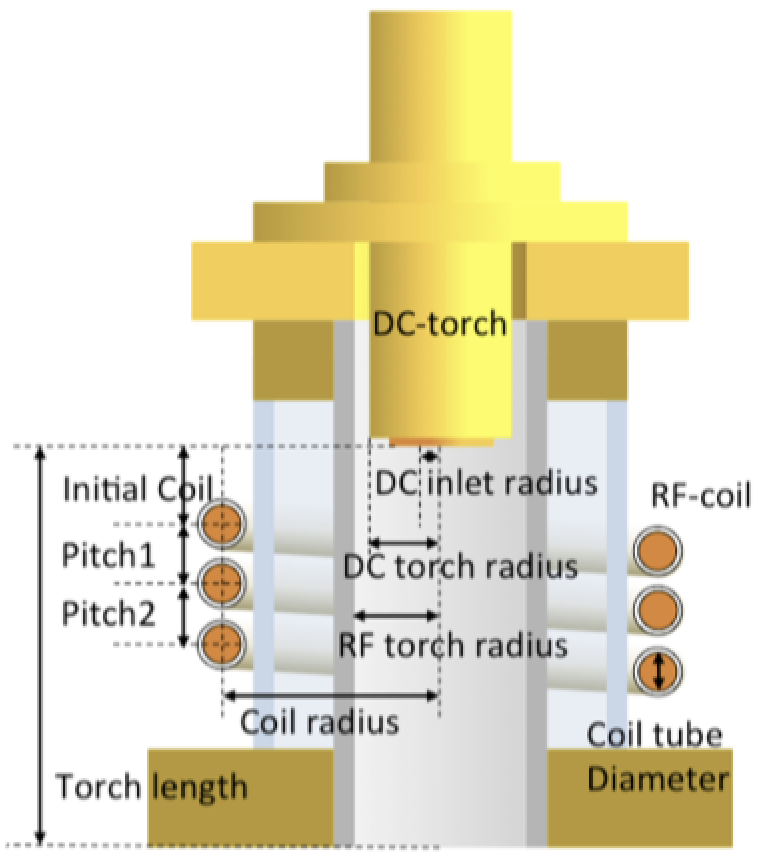
\includegraphics[width=8cm]{src/fig/fig21.png}
\caption{The schematic illusion of a hybrid torch}
\end{figure}

\begin{table}[htbp]
\centering
\caption{ Torch condition}
\begin{tabular}{cc}
\toprule
Parameter & Value\\
\midrule
DC inlet radius(mm) & 4 \\
DC torch radius(mm) & 20 \\
RF torch radius(mm) & 21 \\
Coil tube diameter(mm) & 8 \\
Initial coil(mm) & 22 \\
Pitch 1(mm) & 21.5 \\
Pitch 2(mm) & 21.5 \\
Torch length(mm) & 98 \\
Coil radius(mm) & 33.5 \\
\bottomrule
\end{tabular}
\end{table}

Metallurgical Si(MG-Si) powder is used as a raw material. Unlike Semiconductor Grade Silicon (SEG-Si) or Solar Grade Silicon(SOG-Si), MG-Si allows impurities(98\%~99\%), so it is much cheaper. The average size of MG-Si particle is 19.2 µm as measured by the laser diffraction / scattering method. The powder feeder used is TWIN 10C POWDER FEEDER from SULZER METECO company. The carrier gas is Ar, introduced radially and tangentially, and the flow rate is set to 3.6 slm. A predetermined amount of Ni powder and Si powder mixture is injected to plasma, they are evaporated and co-condensed on the copper plate at the bottom of reactor. 
\subsection{PS-PVD condition}
\begin{table}[H]
\centering
\caption{PS-PVD condition}
\begin{tabular}{cc}
\toprule
Parameter & Value\\
\midrule
Torch diameter(mm) & 60 \\
Torch length(mm) & 150 \\
DC power(kW) & 8 \\
RF power(kW) & 90 \\
DC Ar(slm) & 10 \\
Tangential Ar(slm) & 140 \\
Radial Ar(slm) & 30 \\
Ni addition(at.\%) & 0,5 \\
Powder feeding rate(g/min) & 1 \\
Chamber pressure(torr) & 400 \\
\bottomrule
\end{tabular}
\end{table}
\section{Plasma Enhanced-CVD}
\subsection{PE-CVD apparatus}
\begin{figure}[H]
\centering
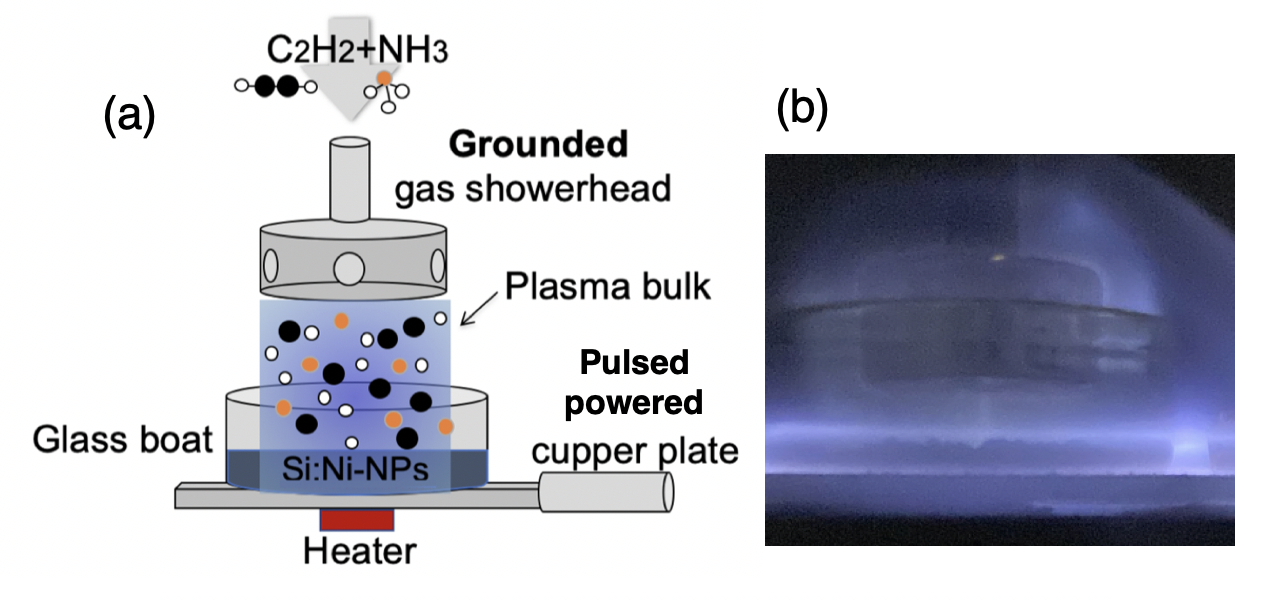
\includegraphics[width=14cm]{src/fig/fig22.png}
\caption{(a)The generation of plasma in PE-CVD.(b)The illustration of Plasma-enhanced CVD.}
\end{figure}
The $\mathrm{C_{2}H_{2}}$ is used as carbon source and $\mathrm{NH_{3}}$ as the dilute gas. The glass boat with a diameter of 3 cm loads the Si:Ni-NP powders and the heater is fixed beneath the copper plate. The power unit to generate plasma is PVM400/DELUX adjustable power supply, of which the output varies from 1 to 20 kV, the frequency varies from 20 to 60kHz and current is up to 25 mA. The micro ceramic heater is MS-1000-10 series from SAKAGUCHI Corp. The maximum temperature of the heater surface can attain 1000\(^\circ\)C at maximum voltage. However, due to the heat dissipation, the actual temperature of copper plate is much lower (350\(^\circ\)C). Initially, we adopted the typical plasma generation method where the gas shower head is grounded and the copper plate is powered. However, once apply RF power on gas shower head , Si:Ni-NP powders exploded due to the discharge. Then we modified the set-up, reversed the electrodes to make it a dielectric-barrier discharge (DBD), with insulating glass boat being the barrier. Finally the explosion problem is solved.There are several parameters that can be controlled to investigate the optimal CNT growth condition: pressure, annealing time, plasma power, flow rate of reacting gases and temperature.

\subsection{CNT growth condition}
\begin{table}[H]
\centering
\caption{Parameters in PE-CVD}
\begin{tabular}{cccc}
\toprule
Parameter          & \multicolumn{3}{c}{Value}                     \\
\midrule
Temperature(\(^\circ\)C)        & 100            & 200           & 300          \\
Pressure(torr)           & \multicolumn{3}{c}{2}                         \\
Electrode distance(cm) & \multicolumn{3}{c}{1}                         \\
Plasma power       & \multicolumn{3}{c}{1$\sim$20kV,20$\sim$60kHz} \\
$\mathrm{C_{2}H_{2}:NH_{3}}$ flow rate(sccm)           & 14:70          & 14:35         & 14:14        \\
Annealing time(min)     & \multicolumn{3}{c}{15}    \\                 \bottomrule  
\end{tabular}
\end{table}

\newpage

\section{Battery assembly}
\begin{figure}[H]
\centering
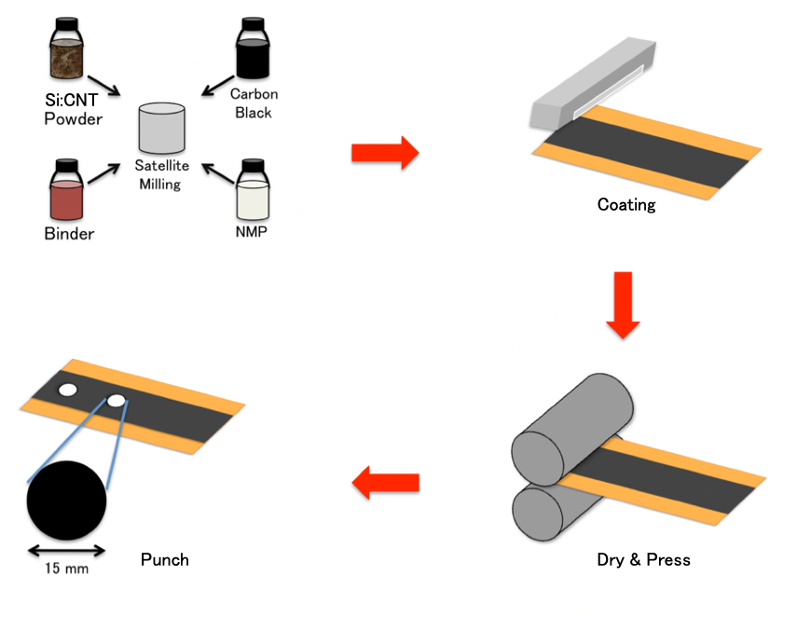
\includegraphics[width=10cm]{src/fig/fig23.png}
\caption{The procedure of battery assembly}
\end{figure}
As shown in Fig. 2.4, the assembly of of a battery can be divided into four steps: slurry preparation, coating, drying and pressing, punching.
\subsubsection{Slurry and milling}
The PS-PVD and PE-CVD processed particles act as the active material in an anode. The particles are sieved to be smaller than 45 um. Then mix with the polyimide binder(25\%), the N-methylpyrrolidone (NMP) solvant (3.3$\sim$4.4 times of the weight of active materials) and carbon black(15\%) in a zirconia container. To well mix them, three zirconia balls with a diameter of 5 mm are put in the container. The container is then centrifuged at 800 rpm for 5 minutes in a centrifuge to produce a slurry. The polyimide binder adheres the active material to the current collector, and the carbon black is conductive material that enhanced the overall conductivity of full cell. NMP was used to adjust the viscosity of the slurry so that the slurry could be applied evenly.
\subsubsection{Coating}
The slurry was applied onto a 12 µm copper foil using a doctor blade for a primary thickness of 75 µm.
\subsubsection{Dry and press}
The slurry on copper foil was then air dried at 110 \(^\circ\)C in an oven, for 15 minutes. In order to improve the adhesiveness and gain uniform thickness, this slurry on copper foil is pressed at 10 kN and dried for another 45 minutes.
\subsubsection{Punch}
The dried slurry is punched into a circle with a diameter of 15 mm so that fits into the coin cell. The mass measured five times and thickness are measured twice.
Figure 2.5 shows the components of a typical half cell. The assembly is operated in a globe box with an inert Ar atmosphere to prevent oxidation of electrodes. The Metal Li is used for the opposite electrode of the half cell. The solvent is Ethylene carbonate and diethyl carbonate with a 1:1 (v:v) ratio. LiPF6 is used as the electrolyte, and a polyolefin porous film is used as the separator. After placing them at the certain sequence, the coin cell case with a rubber gasket is punched by a caulking machine.
\begin{figure}[H]
\centering
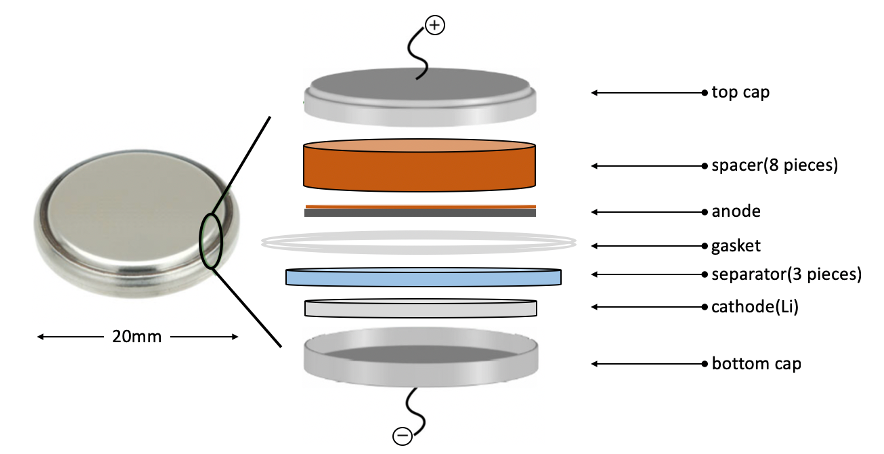
\includegraphics[width=10cm]{src/fig/fig24.png}
\caption{Configuration of  a half cell}
\end{figure}
\section{Powder characteristics}
\subsection{X-ray diffraction (XRD)\textsuperscript{[24]}}
The X-ray diffraction (XRD) was used to determine the crystallographic structure of the phases present and to determine if any preferred orientation (or texture) was present in the materials. If the powder is placed in the path of a with specific X-ray beam of a constant wavelength $\lambda$, Rayleigh scattering occurs and certain diffraction will occur from the planes in those crystallites that are oriented at the correct angle to fulfill the Bragg law.
The Bragg law is,
$$n\lambda=2dsin\theta$$
$d$ is the inter planar spacing of a crystal, $n$(an integer) is the order of reflection, and $\theta$ is the diffraction incident angles.
\begin{figure}[H]
\centering
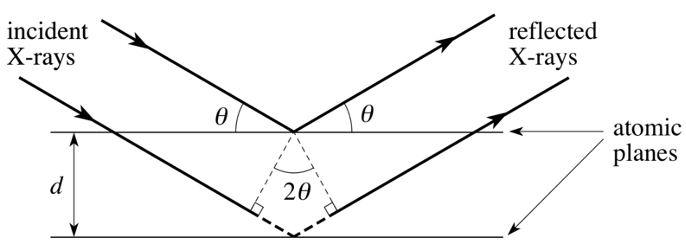
\includegraphics[width=8cm]{src/fig/fig25.png}
\caption{The reflection of Bragg's Law\textsuperscript{[24]} }
\end{figure}
The basic configuration of XRD consists of an X-ray generator, an X-ray filter, a goniometer, a detector, a pulse height analyzer, and a counting circuit. The X-ray generator consists of an X-ray tube class for generating primary X-rays and a power supply that applies a high voltage. The thermions from the tungsten filament kept at a high negative potential are accelerated and collide with the negative electrodes such as Cu, Fe, and Co to emit their characteristic X-rays ($K_\alpha$).  
In this experiment, the $\mathrm{D_{2}}$ PHASER (Bruker Corp.) instrument was
used. Figure 2.11 is a configuration  of X-ray diffraction measurement. A piece of sample is placed in the center of the goniometer. By moving the shutter ,the constantly running X-rays reaches the sample in a specific angle. The sample holder  rotate at certain speed so the to adjust the incident X-ray for diffraction. 
\begin{figure}[H]
\centering
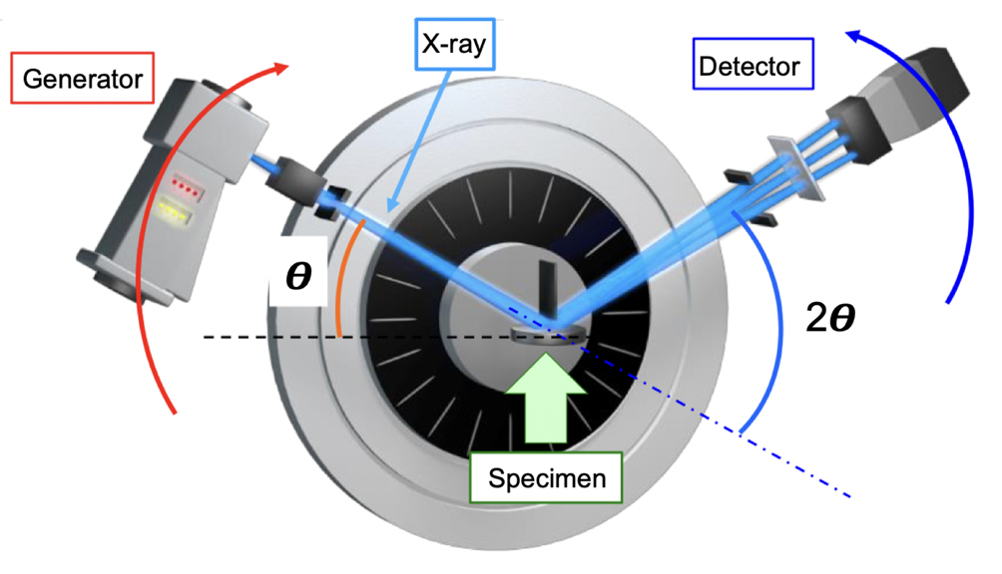
\includegraphics[width=8cm]{src/fig/fig26.png}
\caption{The configuration of XRD instrument\textsuperscript{[25]}}
\end{figure}

\begin{table}[H]
\centering
\caption{XRD condition}
\begin{tabular}{cc}
\toprule
Parameter              & Value                                        \\
\midrule
X ray generating power & 30 kV - 10 mA                                  \\
DS                     & 1 mm                                          \\
Primary solar slit     & $2.5^{\circ}$                                         \\
Secondary solar slit   & $2.5^{\circ}$                                         \\
Diffraction method     & $\mathrm{2\theta /\theta}$  \\
Step size              & $0.02^{\circ}$                                        \\
Scan speed             & 1.0 sec/step    \\                      \bottomrule      
\end{tabular}
\end{table}
\subsubsection{Rietveld analysis\textsuperscript{[26][27]}}
Rietveld analysis is a technique that has been developed for solving/refining crystal structures from powder diffraction data. The method takes a trial structure, calculates a powder diffraction profile and compares it to the measured profile. The trial structure is modified by changing various refinable parameters, including atomic positions, thermal parameters, site occupancies, peak shape parameters, etc., until a best-fit match is obtained with the measured pattern.  Rietveld analysis is especially useful in  quantitative crystalline phase analysis. However, it presents difficulties in quantitative determination of the fraction of the material amorphous part. This way, quantitative percentage of crystalline phases, determined by Rietveld Method, are relative, not considering the amorphous phase, namely,  amorphous carbon in our case.

\subsection{Size distribution\textsuperscript{[28]}}
Laser diffraction is a widely used particle sizing technique for materials ranging from hundreds of nanometers up to several millimeters in size. The way for it to  measures particle size distributions is to measure the angular variation in intensity of light scattered as a laser beam passes through a dispersed particulate sample. It is known that large particles scatter light at small angles and small particles scatter light at large angles. The angular scattering intensity data is analyzed to calculate the size of the particles responsible for creating the scattering pattern, using the Mie theory of light scattering. The particle size is reported as a volume equivalent sphere diameter.

In this experiment, WINGSALD7100 device of  Shimadzu Corporation is employed for particle size distribution measuring. In the work, a highly monochromatic ultraviolet region laser ($\lambda$= 375 µm) generated from a semiconductor laser source is used, and after converting to a parallel beam with a collimator, the particle group is irradiated. The scattered light from this group of particles up to a wide angle of 60 ° is collected by the lens, and concentric diffracted / scattered circles are formed on the detection surface at the focal length. This image is detected by a detector (Wing sensor). In addition, not only the front but also the lateral and rear diffracted light are detected. The particle size distribution is then calculated based on Fraunhofer’s diffraction theory and Mie’s scattering theory.
\begin{figure}[h]
\centering
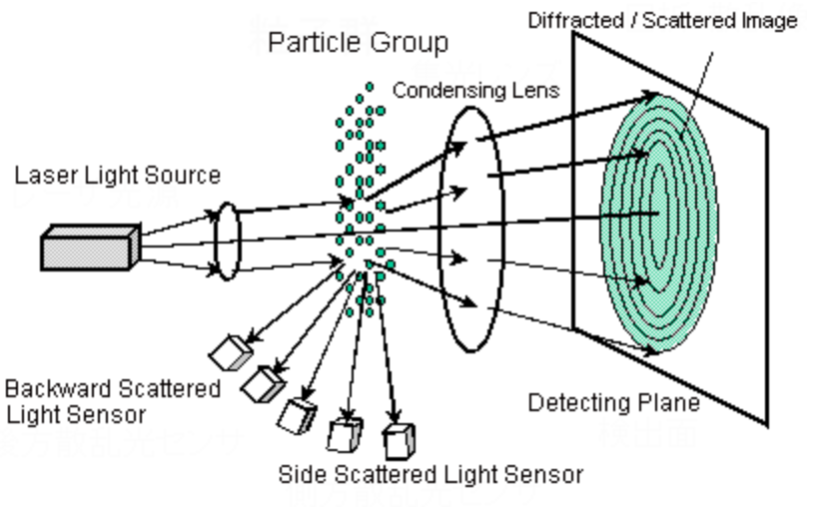
\includegraphics[width=8cm]{src/fig/fig27.png}
\caption{The configuration of laser diffraction system}
\end{figure}

\subsection{Scanning Electron Microscope(SEM)\textsuperscript{[29][30]}}
The Scanning Electron Microscope (SEM) is used for observation of specimen surfaces. When the specimen is irradiated with a fine electron beam (called an electron probe), secondary electrons are emitted from the specimen surface. Morphology of the sample surface can be observed by two-dimensional scanning of the electron probe over the surface and acquisition of an image from the detected secondary electrons. The SEM requires an electron optical system to produce an electron probe, a specimen stage to place the specimen, a secondary-electron detector to collect secondary electrons, an image display unit, and an operation system to perform various operations (Fig. 2.12). The electron optical system consists of an electron gun, a condenser lens and an objective lens to produce an electron probe, a scanning coil to scan the electron probe, and other components. This system (inside of the microscope column) and a space surrounding the specimen are kept in vacuum.
\begin{figure}[H]
\centering
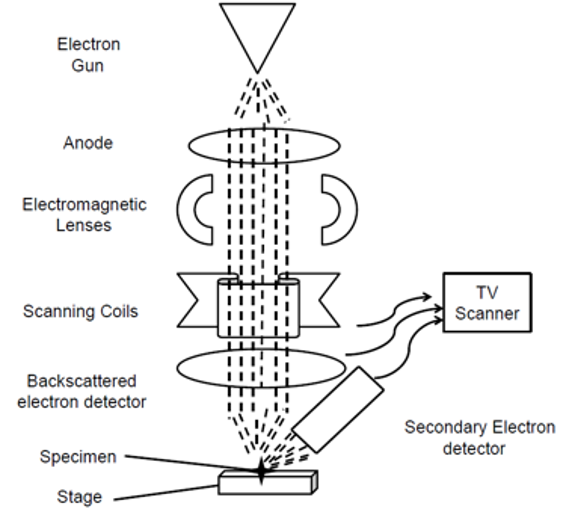
\includegraphics[width=8cm]{src/fig/fig28.png}
\caption{The electron optical system of SEM\textsuperscript{[28]}}
\end{figure}
In this experiment, S-4200 FIELD EMISSION SEM of HITACHI is used.
\subsubsection{Energy Dispersive Spectroscopy(EDS)\textsuperscript{[31]}}
The EDS is used to analyze characteristic X-ray spectra by measuring the energies of the X-rays. When the X-rays emitted from the specimen enter the semiconductor detector, electron-hole pairs are generated whose quantities correspond to the X-ray energy. Measuring these quantities (electric current) enables you to obtain the values of X-ray energy. The detector is cooled by liquid nitrogen, in order to reduce the electric noise. The advantage of the EDS is that the X-rays from a wide range of elements from B to U are analyzed simultaneously. 
\subsection{Raman Spectroscopy\textsuperscript{[32]}}
Raman is a light scattering technique, whereby a molecule scatters incident monochromatic light from a high intensity laser light source. Most of the elastic scattered light is at the same wavelength (or color) as the laser source and does not provide useful information – this is called Rayleigh Scatter. However a small amount of light (typically 0.0000001\%) is inelastic scattered at different wavelengths (or colors), the interaction between the phonons and the laser light results in a shift in energy, and this shift provides information about the modes of phonons in the system, namely, the rotational, vibrational, and other modes of a system.
\begin{figure}[H]
\centering
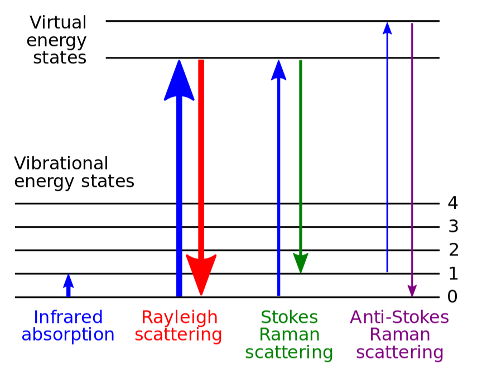
\includegraphics[width=8cm]{src/fig/fig29.png}
\caption{The energy-level diagram of  in Raman spectroscopy\textsuperscript{[33]}}
\end{figure}
If the emitted radiation is of lower frequency than the incident radiation, then it is called Stokes scattering.  If it is of higher frequency, then it is called anti-Stokes scattering. Though any Raman scattering is very low in intensity, the Stokes scattered radiation is more intense than the anti-Stokes scattered radiation. The reason for this is that very few molecules would exist in the excited level as compared to the ground state before the absorption of radiation. Information on the population of a phonon mode is given by the ratio of the Stokes and anti-Stokes intensity of the spontaneous Raman signal. 
\subsection{Transmission electron microscopy(TEM)\textsuperscript{[34]}}
Transmission electron microscopy (TEM) is the original form of electron microscopy and analogues to the optical microscope. It can achieve a resolution of ~0.1 nm, thousand times better resolution, cannot be reached by the light microscope. The beam of electrons passes through the specimen and analyzes the internal structure of the specimen in the form of images. The electron has the poor penetrating capability and gets absorbed in the thick specimen. Therefore, the thickness of the specimen should not be more than few hundred Angstroms ($10^{-10}$ m).  TEM provides information in the form of variations of electron intensity in the image. The electron image is monochromatic and must be made visible to the eye either by allowing the electrons to fall on a fluorescent screen fitted at the base of the microscope column or by capturing the image digitally for display on a computer monitor.
\begin{figure}[H]
\centering
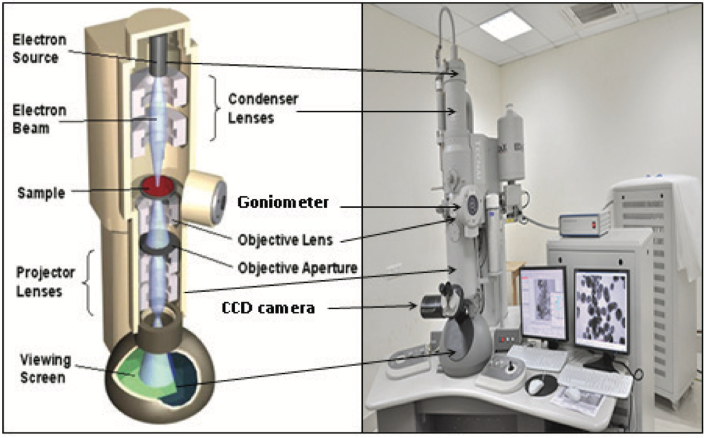
\includegraphics[width=8cm]{src/fig/fig30.png}
\caption{The electron beam system in TEM\textsuperscript{[34]}}
\end{figure}
In this research, the JEM-2010F (acceleration voltage = 200 kV, field emission gun, Tietz F416 camera) is used.
\subsection{Battery  test}
The impedance is an important factor that determines a LIB good or not.  The ex-situ impedance test is carried out with a frequency response analyzer (Solartron1260), an electrochemical interface (Solartron 1287). Set DC Potential as 0 (vs. Open Circuit) and AC amplitude as 10mV. The starting frequency is 1E-6 Hzand it ends at 0.1 Hz. The interval is set to be 10.  The impedance test is performed before charge/discharge service. The impedance is shown in Nyquist plot, in which the data from each frequency point is plotted by theimaginary part on the ordinate and the real part on the abscissa. There are many method to fit the Nyquist plot to do quantitative analysis of impedance. But In this research, qualitative analysis is done by comparing the radius of semicircle, which is enough to tell the good or bad conductivity of a half cell.

The capacity of a battery is expressed as the amount of electricity that can be taken out by discharging a battery charged under certain conditions under certain conditions and reaching the discharge end voltage, so it is affected by the charging / discharging method. Therefore, it is necessary to set appropriate charge / discharge conditions.

In this study, the ACD-01 charge / discharge tester manufactured by Asuka Electronics Co., Ltd. was used as the battery tester. In the battery test, charging and discharging were performed by the constant current method (CC) in which the cutoff voltage was set. Generally, the C rate is used to represent the charge / discharge current value. 1 C means the current value when the capacity of the battery is discharged in 1 hour. Similarly, 0.5 C discharges in 2 hours and 0.1 C discharges in 10 hours. This time, a charge / discharge test was conducted under the conditions of a cut-off voltage of 1.5 V to 0 V, 0.02 C for the initial 3 cycles, and 0.1 C for the 4th and subsequent cycles.


\chapter{Modeling \& Simulation}
\section{Si:Ni-NPs formation }
\subsection{Homogenous nucleation\textsuperscript{[35][37]}}
In PS-PVD process, the Si and Ni powders are fed into plasma and evaporated immediately due to high temperature (>10,000K). Then, Si gas and Ni gas are co-condensed at the tail of plasma (2000$\sim$3000K). In particle formation, nucleation is the first and determining step. A Homogeneous nucleation occurs without any favorable nucleation site while heterogeneous nucleation occurs at a foreign surface. The necessary  physical quantities  and the corresponding symbol used in calculations in this chapter is demonstrated in and Table 3.1.
\begin{table}[h]
\caption{Physical quantity}
\centering
\begin{tabular}{ccc}
\toprule
Symbol & Physical quantity      & Dimension \\
\midrule
$I$    & Nucleation   frequency & $\mathrm{/m^{3}s}$    \\
$\alpha _{i}^{\ast }$ & Adsorption coefficient & -         \\
$S$  & Saturation ratio       & -         \\
$P_{\infty }$ & Saturation pressure    & Pa \\
 $k$ & Boltzmann constant     & J/K       \\
$T$  & temperature            & K         \\
 $\sigma $  & Surface energy   & $\mathrm{J/m^{2}}$\\
$m$ & Molecular mass         & kg        \\
$\rho $& Mass density           & $\mathrm{kg/m^{3}}$     \\
$n_{i}^{\ast }$ & critical density & /$\mathrm{m^{3}}$ \\
$r^{\ast }$ & critical radius & m \\
$L$ & Evaporation latent heat & J/mol \\
\bottomrule
\end{tabular}
\end{table}

\begin{table}[H]
\caption{Physical property\textsuperscript{[36]}}
\centering
\begin{tabular}{ccccccc}
\toprule
Atom & $T_{m}$(K) & $T_{b}$(K) & $\sigma$(mN/m)  & $\rho $($\mathrm{g/cm^{3}}$) & m(g/mol) & L(kJ/mol)\\
\midrule
Si   & 1680 & 3507 & 865  & 2.51 & 28.1 & 386 \\
Ni   & 1726 & 3110 & 1778 & 7.91 & 58.7 & 372\\
\bottomrule
\end{tabular}
\end{table}
There are two rival nucleation theories- the classical Becker-Doring theory and the revised Lothe-Pound theory. According to Becker-Doring theory, the nucleation frequency is  given by:
\begin{equation}
I=\frac{\alpha_{i}^{*} S P_{\infty}}{k T} \sqrt{\frac{2 \sigma}{\pi m}} \frac{m}{\rho} n_{i}^{*}  
\tag{3.1.1}
\end{equation}
The critical density $n_{i}^{\ast }$ is expressed as,
\begin{equation}
n_{i}^{*}=n_{1} \exp \left(-\frac{\Delta G^{*}}{k T}\right) 
\tag{3.1.2}
\end{equation}
where $n_{1}$ is the total number of atoms in the mother phase and $\Delta G^{*}$ is the energy barrier that an atom has to pass over in order to nucleation.
The occurrence of atomistic level events with the length scales on the order of $\sim$0.1 manometers and time scales of $10^{-13}$ seconds makes the nucleation a very complicated phenomenon to study. The  revised Lothe-Pound theory has taken the translational and rotational components of  the free energy of formation in to consideration.  By introducing a correction factor $\Xi_{i}^{*} $  , the critical density $n_{i}^{*}$ is given by following equation:
\begin{equation}
n_{i}^{*}=n_{1} \Xi_{i}^{*} \exp \left(-\frac{\Delta G^{*}}{k T}\right)  
\tag{3.1.3}
\end{equation}
With the expressions above, it has been possible to obtain an understanding of both homogeneous and heterogeneous nucleation. Based on our experiment, we focus the liquid-solid equilibrium system.
When a homogeneous nucleation takes place, there is a transformation from a small bubble of liquid to solid state, wherein two contributions to the change in the energy of the system: the energy decreases because the Gibbs energy of solid ($G_{S}$)  is lower than the energy of the liquid($G_{L}$) ; the energy increase is due to the birth of interface between the liquid and the vapor. The algebraic sum of such decrease and  increase is found to be the driving force for a nuclei formation. It shall be mentioned that the nucleation takes place at constant pressure and temperature.
The algebraic sum of  energy change during homogeneous nucleation is given by:
\begin{equation}
\Delta G=\frac{4 \pi r^{3}}{3} \Delta G_{V}+4 \pi r^{2} \sigma  
\tag{3.1.4}
\end{equation}
Where $r$ is the spherical nucleus of radius and $\sigma $ is the surface energy.
\begin{figure}[H]
\centering
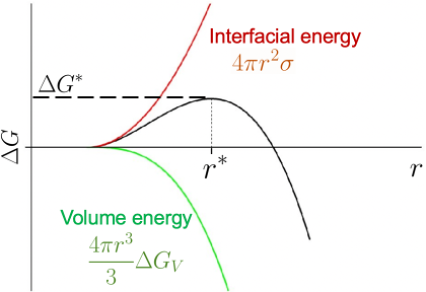
\includegraphics[width=8cm]{src/fig/fig31.png}
\caption{The energy change in nucleation\textsuperscript{[37]}}
\end{figure}
The total energy at first increases with increasing radius before reaching a maximum value at a critical radius $r^{*}$ and then decreasing (see Fig.3.1). The critical radius can be obtained by differentiating $\Delta G$ with respect to $r$, 
\begin{equation}
\frac{d \Delta G}{d r}=4 \pi r^{2} \Delta G_{V}+8 \pi r \sigma=4 \pi r\left(r \Delta G_{V}+2 \sigma\right)=0
\tag{3.1.5}
\end{equation}
By solving this,  $r^{*}$ is
\begin{equation}
r^{*}=-\frac{2 \sigma}{\Delta G_{V}}
\tag{3.1.6}
\end{equation}
Next,  we deal with the $\Delta G_{V}$ term.
The volumetric energy loss is:
\begin{equation}
\Delta G_{V}=G_{L}-G_{S}=H_{L}-H_{S}-T\left(S_{L}-S_{S}\right)
\tag{3.1.7}
\end{equation}
Where the $H$ is enthalpy and $S$ is entropy. Since phase transformation occurs at melting point $T_{m}$, that is, $\Delta G_{V}=0$. With denoting $H_{L}-H_{S}=\Delta H_{m}$, $S_{L}-S_{S}=\Delta S_{m}$, the term of $\Delta H_{m}$ equals  $T_{m}\Delta S_{m}$  at melting point.  Assume $\Delta H_{m}$ and $\Delta S_{m}$  are independent from temperature. Since nucleation needs driving force thus some overcooling is necessary.  
The derivation of above equations is,
\begin{equation}
\Delta G_{V}=\Delta H_{m}-T \Delta S_{m}=\Delta H_{m}-T \cdot \frac{\Delta H_{m}}{T_{m}}=\Delta H_{m} \frac{\Delta T}{T_{m}}
\tag{3.1.8}
\end{equation}
Substituting this expression into the eqn.(3.5) we get,
\begin{equation}
r^{*}=-\frac{2 \sigma T_{m}}{\Delta H_{m} \Delta T}
\tag{3.1.9}
\end{equation}
It’s clear that only a system with larger overcooling degree will be able to sustain a stable nucleation. 
Based information above, the energy barrier for a homogeneous nucleation is, 
\begin{equation}
\Delta G^{*}=\frac{16 \pi \sigma^{3}}{3 \Delta G_{V}^{2}}=\frac{16 \pi \sigma^{3} T_{m}^{2}}{3 \Delta H_{m}^{2} \Delta T^{2}}=\frac{4 \pi \sigma}{3}\left(r^{*}\right)^{2}
\tag{3.1.10}
\end{equation}
Here, the Kelvin equation is introduced to give the another expression of $r^{*}$ based on saturation mechanism.
\begin{equation}
r^{*}=\frac{2 \sigma v}{k T \ln S}
\tag{3.1.11}
\end{equation}
Here, $v$ is the volume of a droplet. Substituting this equation back with the assumption that $I =10^{22}$ ,  Then apply eqn.(3.1.2),(3.1.10),(3.11) into (3.1.1) ,  the following balance equation can be derived.
\begin{equation}
(\ln S)^{3}+\left(\frac{1}{2} \ln \left(\frac{\alpha_{i}^{*} P_{\infty}^{2} \Xi_{i}^{*}}{(k T)^{2} \rho I} \sqrt{\frac{2 \sigma m}{\pi}}\right)\right)(\ln S)^{2}-\frac{8 \pi \sigma^{3} v^{2}}{3(k T)^{3}}=0
\tag{3.1.12}
\end{equation}
We adopt the  $\Xi_{i}^{*}=10^{17}$ suggested by Lothe and Pound and assume adsorption coefficient  be 1, the $S$ can be calculated by applying all the physical properties shown in table 3.2. We denote this $S$ from calculation as theoretical value $S_{th}$.
On the other hand, $S$ can be expressed by its definition based on experimental condition. Assume at the time Si and Ni powders are fed into plasma they are evaporated immediately. Let partial pressure of each element, which can be calculated by feeding rate and chamber pressure, divide the corresponding theoretical saturated vapor pressure, we get the supersaturation $S_{n}$ experimentally\textsuperscript{[38]}.
Since both $S_{th}$ and $S_{n}$ are the functions of temperature, the intersection of two curves becomes the nucleation temperature. 
\begin{figure}[H]
\centering
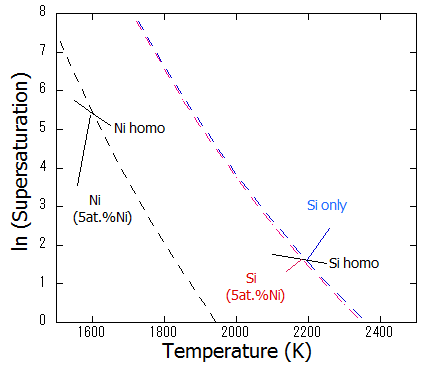
\includegraphics[width=8cm]{src/fig/fig32.png}
\caption{The homogeneous nucleation of Si and Ni in PS-PVD.}
\end{figure}

\begin{table}[H]
\caption{Homogeneous nucleation temperature of Si and Ni}
\centering
\begin{tabular}{ccc}
\toprule
Ni addition(at.\%) & $T_{N}^{Homo,Si}$(K) & $T_{N}^{Homo,Ni}$(K)     \\
\midrule
0                  & 2190 & -    \\
5                  & 2183 & 1604 \\
\bottomrule
\end{tabular}
\end{table}

\subsection{Heterogeneous nucleation\textsuperscript{[39]}}
The discussion so far has considered the homogeneous nucleation, which occurs spontaneously and randomly but requires supercooling.  In contrast,  heterogeneous nucleation occurs much more often in PS-PVD system because at some preferential sites, the effective surface energy is lower, thus diminishes the free energy barrier and facilitating nucleation. 
When heterogeneous nucleation occurs, to be specific, a cap-shaped liquid droplet  is deposited onto a solid surface, it will form a contact angle depending on its on surface tension as shown in fig.3.3
There are three different surface energies of interest:
\begin{itemize}
  \item $\sigma_{S L}^{A B}=(\text { solid } A-\text { liquid } B)$
  \item $\sigma_{L V}^{B}=(\text { vapor } \text { liquid } B)$
  \item $\sigma_{S V}^{A}=(\text { solid } A-\text { vapor })$
\end{itemize}
\begin{figure}[H]
\centering
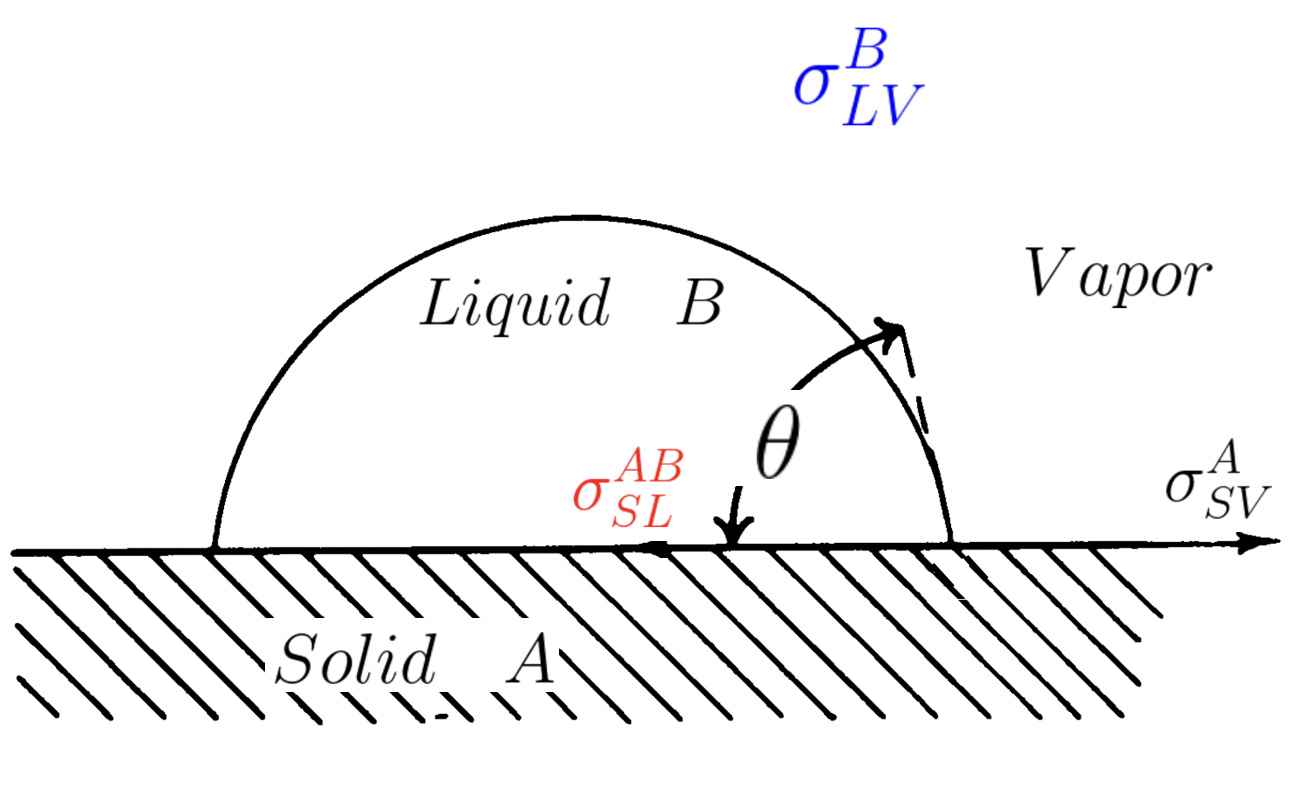
\includegraphics[width=8cm]{src/fig/fig33.5.png}
\caption{Surface tension}
\end{figure}
The contact angle $\theta $ can be  derived  in following equations:
\begin{equation}
\cos \theta=\frac{\sigma_{L V}^{A}}{\sigma_{L V}^{B}}-\frac{\lambda}{L_{e}^{B}}
\tag{3.1.13}
\end{equation}
Where  the $ \lambda $ represents solubility parameter and $L$ is the enthalpy of solution.
\begin{table}[H]
\caption{Enthalpy of solution\textsuperscript{[39]}}
\centering
\begin{tabular}{ccc}
\toprule
Solute & Solvent & Enthalpy of solution(kJ/mol) \\
\midrule
Si     & Ni      & -98                          \\
Ni     & Si      & -86                          \\
\bottomrule
\end{tabular}
\end{table}
According to Table 3.4,  we have  $ \lambda $ of -92 kJ/mol, which is the average of two enthalpies listed. 
Using the property values in Table 3.2 and Table 3.4, the contact angle of Ni droplet on a Si flat plane is,
\begin{equation}
\cos \theta=0.734
\tag{3.1.14}
\end{equation}
With the assumption that the surface energy of solid silicon is equal to liquid silicon. Next, consider the energy barrier for a heterogeneous nucleation. Here introduce the concept of shape factor,
\begin{equation}
f(\theta)=\frac{\cos ^{3} \theta-3 \cos \theta+2}{4}
\tag{3.1.15}
\end{equation}
With the same radius and same undercooling, the energy change by heterogeneous nucleation differs by such shape factor located outside the brackets of eqn.(3.4).
\begin{equation}
\Delta G=\left(\Delta G_{v} \frac{4}{3} \pi r^{3}+\sigma_{L V} 4 \pi r^{2}\right) \frac{\cos ^{3} \theta-3 \cos \theta+2}{4}
\tag{3.1.16}
\end{equation}
It is noteworthy that the critical radius $r^{*}$ remains unchanged for heterogeneous nucleation and homogeneous nucleation. Thus, the nucleation frequency $I$ can be expressed as,
\begin{equation}
I=\frac{\alpha_{i}^{*}\left(S P_{\infty}\right)^{2}}{(k T)^{2} \rho} \sqrt{\frac{2 \sigma m}{\pi}} \Xi_{i}^{*} \exp \left(-\frac{16 \pi \sigma^{3} v^{2}}{3(k T)^{3}(\ln S)^{2}} f(\theta)\right)
\tag{3.1.17}
\end{equation}
With the same assumption that $I =10^{22}$  and same substitution procedure in homogeneous case, the theoretical $S$ of  heterogeneous nucleation can be calculated .
However, this calculation is based on the simplification that Si particle surface is flat with respect to the heterogeneously formed nuclei. Practically, in the case of this PS-PVD experiment, Ni droplet is  expected to nucleate on solid Si nanoparticle in a spherical shape as fig.3.4 shows. 
\begin{figure}[H]
\centering
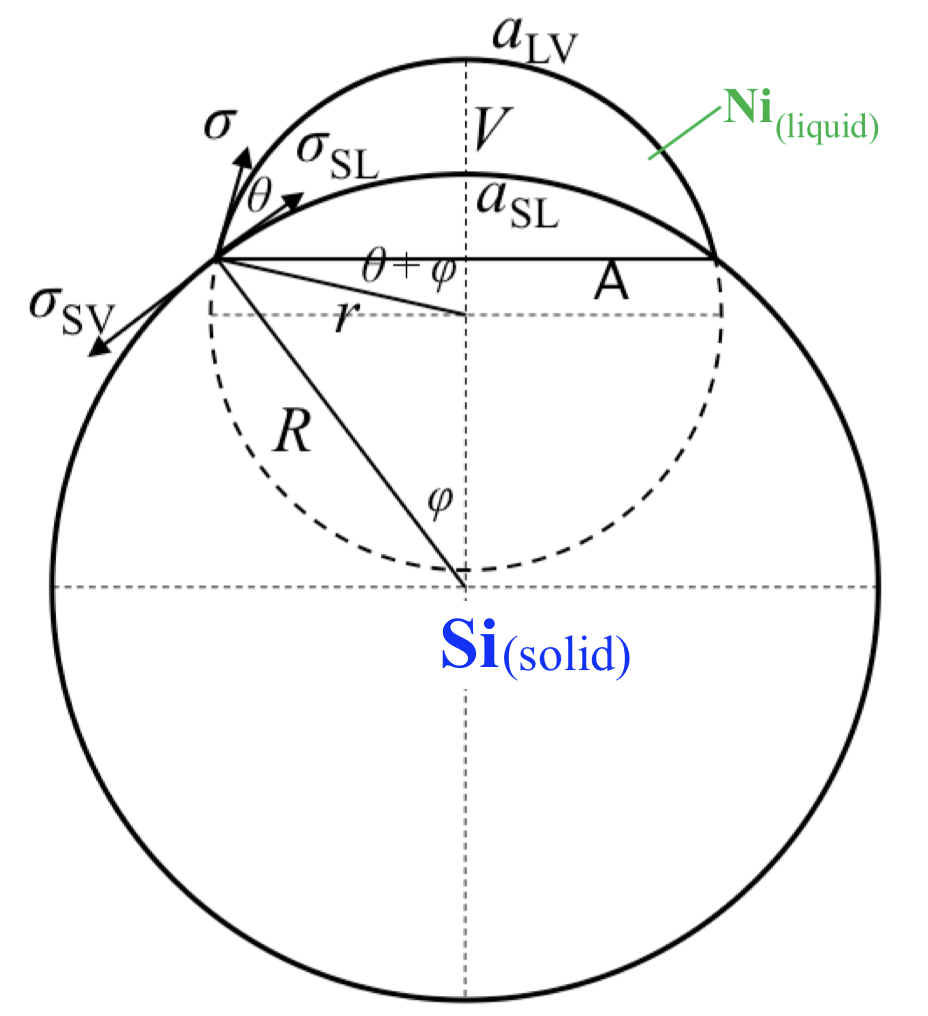
\includegraphics[width=8cm]{src/fig/fig33.png}
\caption{Schematic of heterogeneous nucleation on nanoparticles\textsuperscript{[40]}}
\end{figure}
As the diameter of Si nanoparticle changes, the shape factor changes accordingly. Fig.3.5 shows the shape factor $f(\theta)$ becomes a function of the diameter of Si nanoparticle, here $r^{*}$ =0.5 nm is assumed.
\begin{figure}[H]
\centering
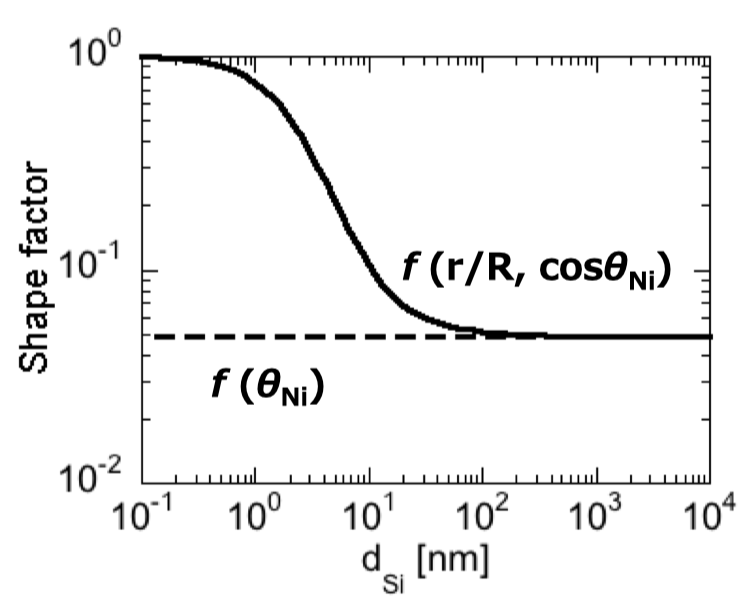
\includegraphics[width=8.5cm]{src/fig/fig34.png}
\caption{The shape factor of Ni on Si nanoparticle in different size}
\end{figure}
Fig.3.5 demonstrate that when $d_{Si}$ in the range of 0.1 $\sim$ 100 nm, shape factor undergoes a sharp drop, and when $d_{Si}$ > 100 nm, the shape factor becomes a constant, that is, $\cos \theta=0.734$, the same with the flat plane case. In addition, it's clear that  when heterogeneous nucleation takes place on smaller Si particles, the shape factor becomes large, and therefore the energy barrier becomes large, adding difficulties for Ni to nucleate on it. By applying different shape factor into calculation, the nucleation points of Ni on different-size Si particle is presented in Figure 3.6. As expected, the smaller Si particle is, the larger overcooling degree is needed for Ni to nucleate.

\begin{figure}[H]
\centering
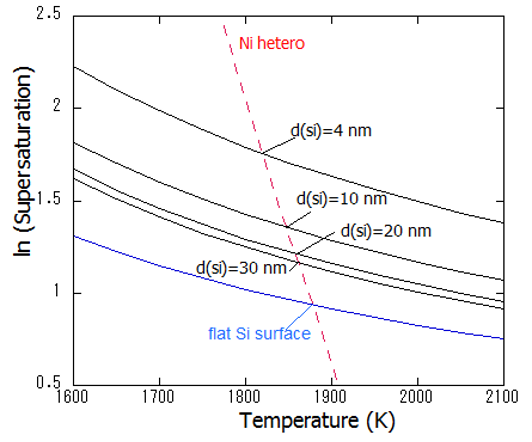
\includegraphics[width=8cm]{src/fig/fig35.png}
\caption{The size dependent heterogeneous nucleation of Ni on Si.}
\end{figure}
In each case the heterogeneous nucleation point of Ni on Si particle is in between $T_{N}^{Homo,Si}$(2183K) and $T_{N}^{Homo,Ni}$(1604K), 
holding the sequence of 
$$\boxed{T_{N}^{Homo,Si}>T_{N}^{Hetero,Ni}>T_{N}^{Homo,Ni}}$$
Only in this sequence can we obtain the target Si:Ni nanostructure.

\subsection{Particle growth\textsuperscript{[36]}}
There are two types of particle growth after nucleation: (1) The coagulation by adsorption of vapour atoms/molecules on the particle surface. (2) The coagulation by collision-coalescence of particles. However, the former is credible only in really initial stages of particle growth, i.e. when their diameters are of order 1 nm. In the case of our PS-PVD processing particle,  such approximations are obviously not possible. Therefore, the latter called collision-coalescence theory is used.

In collision-coalescence theory, there are two approaches: (1) the Collision Rates Continuum Theory, which is treated as a diffusion problem, and (2) the Free Molecule Theory based on the noble gas particle kinetics.  When the ratio of mean free path to particle radius is <0.1, the former is used.  If such ration >10, the latter is used. In our case, the mean free path is $\sim$850 nm, as will be described later, so the Free Molecule Theory can be applied for particle size up to 140 nm. From the experimental results, the primary particle size  satisfy this size requirement, the  Free Molecule Theory  is used.

In a system of  three classes of gases colliding with each other, the mean free path of  particular gas 1  can be expressed as,

\begin{equation}
\begin{split}
\lambda_{1 \rightarrow 1,2,3} &= \frac{\bar{c}_{1}}{\Gamma_{1 \rightarrow 1,23}}\\
&=\frac{1}{\pi\left(\sqrt{2} \sigma_{1}^{2} N_{1}+\left(\frac{\sigma_{1}+\sigma_{2}}{2}\right)^{2} N_{2} \sqrt{1+\frac{m_{1}}{m_{2}}}+\left(\frac{\sigma_{1}+\sigma_{3}}{2}\right)^{2} N_{3} \sqrt{1+\frac{m_{1}}{m_{3}}}\right)}\\
\end{split}
\tag{3.1.18}
\end{equation}
Where $c$ represents the speed, $\sigma $ represents the collision diameter, $\Gamma $represents the collision frequency.
Apply the collision diameter listed in table3.? to equation the mean free path  of Si can be  obtained. $\lambda_{Si}=\sim 850$ nm. To satisfy the Free molecule theory the Si particle should be smaller than 170 nm. In addition, it’s difficult for Ar or H atom to be included into a Si particle, so we can just focus on the case of Si collide with each other. Then $\lambda_{Si}$ can be reduced to $\sim 400 \mu m$. This enlarge the requiring Si particles size to several micro meters. 

\begin{table}[H]
\caption{collision diameter\textsuperscript{[37]}}
\centering
\begin{tabular}{cc}
\toprule
Molecule &  $\sigma$(\AA) \\
\midrule
Si       & 3.046 \\
Ar       & 3.432 \\
H        & 2.915 \\
\bottomrule
\end{tabular}
\end{table}
Next, consider the collision between larger particles. 
The collision frequency of particles consisting of i atoms and particles consisting of j atoms is,
\begin{equation}
L_{i j}=\left(8 \pi k T \frac{m_{i}+m_{j}}{m_{i} m_{j}}\right)^{\frac{1}{2}}\left(R_{i}+R_{j}\right)^{2} N_{i} N_{j}
\tag{3.1.19}
\end{equation}
Where $m$ is the mass, $R$ is the radius and $N$ is the particle number concentration.
Differentiating $N$ with respect to $t$(time) gives,
\begin{equation}
\frac{d N}{d t}=\sum_{i=1}^{\infty} \frac{d N_{i}}{d t}=c\left(\sum_{i=1}^{\infty} \sum_{j=1}^{i-1} \frac{1}{2} L_{j(i-1)}+\frac{1}{2} \sum_{i=1}^{\infty} L_{ii}-\sum_{i=1}^{\infty} \sum_{j=1}^{\infty} L_{i j}\right)
\tag{3.1.20}
\end{equation}
$c$ represents the sticking coefficient.
Assume the particles are the same size,to say, $i = j$.  eqn. (3.20) can be rewritten as:
\begin{equation}
\frac{d N}{d t}=-\frac{c}{2}\left(\frac{16 \pi k T}{m}\right)^{\frac{1}{2}}(2 R)^{2} N^{2}
\tag{3.1.21}
\end{equation}
Note that the following relationships  constantly hold:
\begin{equation}
m=\frac{4}{3} \pi R^{3} \rho
\tag{i}
\end{equation}
\begin{equation}
N=\frac{3 C_{0} M}{4 \pi R^{3} \rho N_{A}}
\tag{ii}
\end{equation}
$C_{0}$  is the concentration of molecules and $m$ is the molecular weight.
Substitute the $m$ and $N$ above into eqn. (3.21) we have,
\begin{equation}
\frac{d N}{d t}=-4 c\left(\frac{3 k T}{\rho}\right)^{\frac{1}{2}}\left(\frac{3 M}{4 \pi \rho N_{A}}\right)^{\frac{1}{6}} C_{0}^{\frac{1}{6}} N^{\frac{11}{6}}
\tag{3.1.22}
\end{equation}
In PS-PVD, the temperature will decrease with time. So we introduce the cooling rate $\varepsilon $ (K/s),
\begin{equation}
T=T_{0}-\varepsilon t
\tag{3.1.23}
\end{equation}
Applying this temperature profile into eqn. (3.22) and by solving this differential equation, the particle number concentration can be obtained.
\begin{equation}
N=N_{0}\left(1+\frac{20 \sqrt{3}}{9} c\left(\frac{k}{\rho}\right)^{\frac{1}{2}}\left(\frac{3 M C_{0}}{4 \pi \rho N_{A}}\right)^{\frac{1}{6}} \frac{1}{\varepsilon}\left(T_{0}^{\frac{3}{2}}-\left(T_{0}-\varepsilon t\right)^{\frac{3}{2}}\right) N_{0}^{\frac{5}{6}}\right)^{-\frac{6}{5}}
\tag{3.1.24}
\end{equation}
However, $\varepsilon $ is a function of time instead a constant. For convenience, an analytical solution is obtained with incorporation of $\varepsilon (t)$ and the assumption of sticking coefficient $c=1$.
The analytical solution  is carried out with setting proper step size of the variable,namely, $t$. In each step size the cooling rate is constant. Let $T_{0}$ and  $T_{1}$ be the initial and final temperature, respectively. And we have the cooling rate as,
\begin{equation}
\varepsilon=\frac{T_{0}-T_{1}}{\Delta t}
\tag{3.1.25}
\end{equation}
By replacing the initial value of $N$ repeatedly, analytical solution of $N$ is obtained. 
Using this particle number concentration, we can calculate the particle size with the relationship between the existing Si atoms, the density of Si atoms in a particle and the volume of a Si atom.
\begin{figure}[H]
\centering
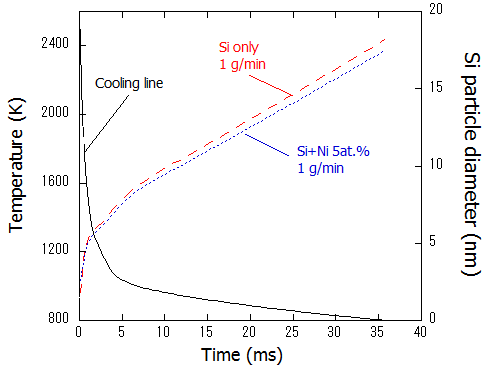
\includegraphics[width=9cm]{src/fig/fig36..png}
\caption{Si particle growth}
\end{figure}
As Fig.3.7 shows, the final diameter of Si primary particle in PS-PVD is 20nm.

\newpage
\section{CNT growth in PE-CVD}
\subsection{Mathematical model of CNT growth\textsuperscript{[41]}}
\begin{table}[H]
\centering
\caption{Physical quantity for CNT growth simulation}
\begin{tabular}{@{}lcc@{}}
\toprule
Description                                                                  & symbol   & unit      \\ \midrule
Initial concentration of feedstock gas                                       & $n_{0}$  & $m^{-3}$  \\
Volumetric number density of  $\mathrm{C_{2}H_{2}}$                             & $n$      & $m^{-3}$  \\
Volumetric number density of pyrolysis product $\mathrm{C_{4}H_{4}}$            & $n_{p}$  & $m^{-3}$  \\
Mass of $\mathrm{C_{2}H_{2}}$                                                & $m$      & kg        \\
Mass of $\mathrm{C_{4}H_{4}}$                                                & $M$      & kg        \\
Surface area of catalyst(Ni) particle                                        & $S_{0}$  & $m^{2}$   \\
Particle flux of  $\mathrm{C_{2}H_{2}}$ to Ni surface                         & $F_{b1}$ & $s^{-1}$  \\
Particle flux of $\mathrm{C_{4}H_{4}}$ to Ni surface                          & $F_{b2}$ & $s^{-1}$  \\
Particle flux of Carbon provided by $\mathrm{C_{2}H_{2}}$                    & $F_{c1}$ & $s^{-1}$  \\
Particle flux of Carbon provided by $\mathrm{C_{4}H_{4}}$                    & $F_{c2}$ & $s^{-1}$  \\
Coefficients relating to $\mathrm{C_{2}H_{2}}$ sticking and geometric process  & $p_{1}$  & -         \\
Coefficients relating to $\mathrm{C_{2}H_{2}}$ sticking and geometric process & $p_{1}$  & -         \\
Carbon atoms on the surface                                                  & $N_{C}$  & -         \\
Carbon atoms converted to carbonaceous layer                                 & $N_{L1}$ & -         \\
Inactive Ni atoms                                                            & $N_{L2}$ & -         \\
Carbon atoms diffused into bulk Ni                                           & $N_{B}$  & -         \\
Carbon atoms incorporated into CNT                                           & $N_{T}$  & -         \\
Rate constant of surface–bulk penetration of Carbon                          & $k_{sb}$ & $s^{-1}$  \\
Rate constant of bulk diffusion of Carbon in Ni                              & $k_{b}$  & $s^{-1}$  \\
Rate constant of aurface diffusion of Carbon on Ni                           & $k_{s}$  & $s^{-1}$  \\
Rate constant of precipitation of carbon into  CNT                           & $k_{t}$  & $s^{-1}$  \\
Rate constant of carbonaceous layer formation                                & $k_{c1}$ & $s^{-1}$  \\
Rate constant of carbonaceous layer dissolution                              & $k_{d1}$ & $s^{-1}$  \\
Number of monolayers in MWCNT                                                & $\alpha$ & -         \\
Number density of Carbon atoms on a monolayer                                & $n_{m}$  & $cm^{-2}$ \\
Number density of Carbon atoms per length                                    & $z$      & $cm^{-1}$ \\ \bottomrule
\end{tabular}
\end{table}
The earliest growth mechanisms of CNTs is established by Baker\textsuperscript{[18]}. In recent decades, several research groups have published many models with a better understanding of the growth mechanisms. They are all more or less based on the same processes, including adsorption and dissolution of carbon species at the metal catalyst particle, surface or bulk diffusion nanostructure nucleation and growth. Most of these models are applied to CNT growth by thermal CVD, but some are applied also for PE-CVD, and in general the principles are the same for both growth techniques.

In the case of Si:Ni-NPs as the substrate to grow CNT, where the Ni is directly attached to Si nanoparticle and it is expected to be the catalyst. However, even plasma is utilized to provide a low-temperature growth condition, this Si:Ni template is different from those in literature, for there is no diffusion barrier in between Si and Ni. That is, Ni silicidation is inevitable at elevated temperature. Therefore,  the Ni atoms will diffuse into Si while CNT grow on Ni, which may early terminate CNT without attain to the expected length.  
For convenience, we first concentrate on the move of carbon atoms, assuming Ni silicidation is not occurred at elevated temperature. Through this way can we establish a fundamental modelling of CNT and thereby revise it with adding the Ni-silicidation effect. 
The CNT growth model is  based on the thermal CVD\textsuperscript{[41]} applying to all temperature range.  By focusing the balance of carbon particles at different location, the length of carbon nanotubes becomes a function of annealing time. There are two competitive processes that contribute to the CNT growth and termination. For positive growth, the feed stock gas $\mathrm{C_{2}H_{2}}$ decompose into carbon atoms that diffuse in catalyst bulk and on surface then incorporate into carbon nanotubes. For negative termination, the excessive decomposed carbon atoms from $\mathrm{C_{2}H_{2}}$ form a carbonaceous layer that reduce the active catalyst surface. Also, a small fraction of $\mathrm{C_{2}H_{2}}$ convert into its pyrolysis product, which contains excessive carbon atoms per molecule. Such pyrolysis product contributes to pyrolysis product. If the temperature is high enough, some extra reactions take place, for instance, catalyst poisoning, that contribute to termination as well. 
\begin{figure}[H]
\centering
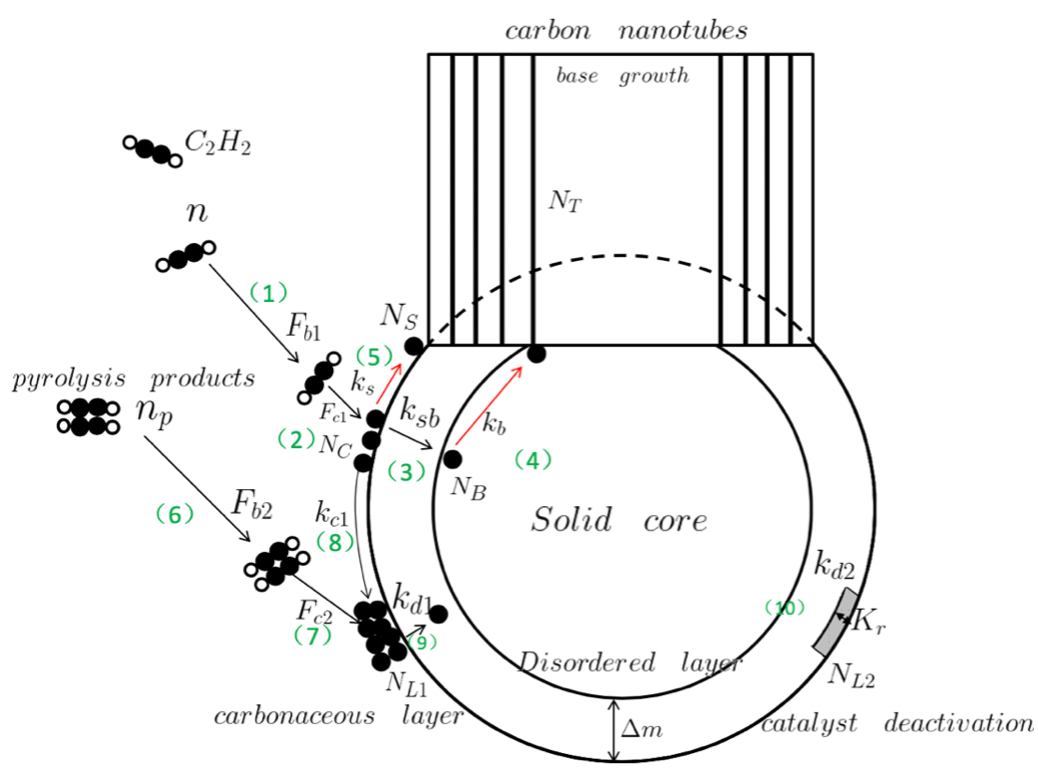
\includegraphics[width=12cm]{src/fig/fig37.png}
\caption{Schematic representation of processes responsible for feeding and termination of CNT growth. The number in bracket represents specific reaction\textsuperscript{[41]}.}
\end{figure}
As Fig.3.8 shows, the moving of carbon-containing species are divided into elementary processes and each are described by a single rate constant in an Arrhenius form.
The catalyst particle is regarded as a sphere, of which the initial surface area is:
\begin{equation}
S_{0}=4 \pi r^{2}
\end{equation}
With the carbonaceous layer forming, the exposed surface is reduced and expressed in terms of effective surface. 
\begin{equation}
S=\left(1-\frac{N_{L}}{\alpha S_{0} n_{m}}\right)S_{0}
\end{equation}
$\alpha $ is the number of monolayers, $n_{m}={10}^{15} m^{-2}$ is the surface density of a monolayer of carbon atoms.
\\
(1) The $\mathrm{C_{2}H_{2}}$  flux physically impinge to catalyst surface $F_{c1}$ following Hertz–Knudsen equation. 
\begin{equation}
F_{b 1}=\frac{1}{4} S_{0} n\left(\frac{k_{\mathrm{B}} T}{2 \pi m}\right)^{1 / 2}
\tag{3.2.1}
\end{equation}
(2) Only a fraction of impinging $\mathrm{C_{2}H_{2}}$ flux can be chemically absorbed and decomposed by catalyst. Assume the coefficients relating to $\mathrm{C_{2}H_{2}}$ sticking and geometric process $p_{1}=1$.  The decomposition reaction, of which the rate constant is $k_{de1}$ and decomposition energy barrier $E_{de1}$ , provides primary carbon atoms $N_{C}$ on the surface of catalyst.
\begin{equation}
F_{c 1}=p_{1}F_{b1}\exp \left(-E_{d e 1} / k_{B} T\right)
\tag{3.2.2}
\end{equation}
Assuming this decomposition is $0^{th}$ order reaction(gas concentration independent), So the decomposition rate constant $k_{de1}$ can be derived as,
\begin{equation}
k_{d e 1}=\frac{S_{0}}{p_{1}} \frac{1}{4} n \sqrt{\frac{k_{B} T}{2 \pi m}} \exp \left(-E_{d e 1} / k_{B} T\right)
\tag{3.2.3}
\end{equation}
(3) Surface-bulk penetration of carbon atoms with the rate constant, $k_{sb}$:
\begin{equation}
k_{s b}=B \exp \left(-E_{s b} / k_{B} T\right)
\tag{3.2.4}
\end{equation}
(4) Bulk diffusion of carbon atoms: the rate determining step in typical thermal CVD. assume that dissolution of carbon atoms will form a highly disordered ‘molten’ layer on the surface with thickness $\delta m$, expressed in the number of carbon monolayers denes the number of CNT walls. Note that the term ’bulk’ refers to the molten layer, because with the assumption of molten layer in between surface and sold core, carbon atoms will not diffuse further into solid core to prevent unnecessary paths. After diffusing and migrating to nucleation site, the carbon atoms $N_{B}$, is absorbed immediately into $N_{T}$ with a kinetic rate constant $k_{b}$. To quantify $k_{b}$ , consider the characteristic time for bulk diffusion[ref6].
\begin{equation}
\tau_{b} \approx l^{2} / D_{b}
\tag{3.2.5}
\end{equation}
where $l$ is the characteristic path length of diffusing species. For a spherical medium $l=r$,  $D_{b}$ is the bulk diffusion coefficient. Thus, the bulk diffusion rate constant $k_{b}$ can be expressed as:
\begin{equation}
k_{b}=\frac{D_{b 0}}{r^{2}} \exp \left(-E_{b} / k_{B} T\right)
\tag{3.2.6}
\end{equation}
(5) Surface diffusion of carbon atoms on catalyst surface, nucleation, and carbon atoms continuous incorporation into $N_{T}$. Generally, before growth can start, nucleation has to take place. If the growth process is the rate controlling step, a continuous acceleration should be observed in the early stages of the deposition. 
\begin{equation}
k_{s}=\frac{D_{s 0}}{r^{2}} \exp \left(-E_{s} / k_{B} T\right)
\tag{3.2.7}
\end{equation}
It’s noteworthy that bulk diffusion(step(3)-(4)) and surface diffusion (5) are parallel routes.  It has been often stated in the literature  that the surface diffusion may be the main processes enabling a rapid, low-temperature growth of CNTs, or more preciesly, CNFs, due to the low temperature. On the contrast,at relatively high substrate temperatures (T>500\(^\circ\)C), the dominant carbon diffusion will be the bulk diffusion. The details is discussed in next section. 

After completing nucleation, a continuous decline in rate would be expected, as the area available for the gas reaction is progressively reduced by the growth of carbon on it. The termination of CNT is determined by excessive carbon atoms that form carbonaceous layer that contains $N_{L1}$ carbon atoms. In addition, at higher temperature  (>700\(^\circ\)C), some mechanisms that are responsible for the catalytic deactivation should be taken into account. For instance, poisoning, due to gas-phase pyrolysis products; formation of metal carbide; catalyst oxidation, etc.
\\

\noindent (6) The carbonaceous layer containing $N_{L1}$ carbon atoms is partly formed by impingement, chemisorption, catalytic decomposition of pyrolysis products. The pyrolysis product can be $\mathrm{C_{4}H_{4}}$, $\mathrm{C_{6}H_{6}}$, etc. For simplification, we consider $\mathrm{C_{4}H_{4}}$ only. This process is the same with step (1), only the subject is different. The impinging  $\mathrm{C_{4}H_{4}}$ flux onto the catalyst surface is,
\begin{equation}
F_{b 2}=\frac{1}{4} S_{0} n_{p}\left(\frac{k_{\mathrm{B}} T}{2 \pi M}\right)^{1 / 2}
\tag{3.2.8}
\end{equation}
(7) The pyrolysis product $\mathrm{C_{4}H_{4}}$ undergoes samely  chemisorption, catalytic decomposition in step(2). Assume coefficient $p_{2}=1$ and denote decomposition energy barrier of pyrolysis product as $E_{de2}$.
\begin{equation}
F_{c 2}=p_{2}F_{b2}\exp \left(-E_{d e 2} / k_{B} T\right)
\tag{3.2.9}
\end{equation}
So the related decomposition rate constant $k_{de2}$ can be derived as,
\begin{equation}
k_{d e 2}=\frac{S_{0}}{p_{2}} \frac{1}{4} n_{p} \sqrt{\frac{k_{B} T}{2 \pi M}} \exp \left(-E_{d e 2} / k_{B} T\right)
\tag{3.2.10}
\end{equation}
(8) Part of $N_{C}$ carbon atoms are integrated into  carbonaceous layer.
\begin{equation}
k_{c l}=G \exp \left(-E_{c l} / k_{B} T\right)
\tag{3.2.11}
\end{equation}
(9) This carbonaceous layer could be partially dissolved by the catalyst.
\begin{equation}
k_{d s 1}=H \exp \left(-E_{d s 1} / k_{B} T\right)
\tag{3.2.12}
\end{equation}
(10) As for the extra reactions at higher temperature, assign a rate constant,$K_{r}$, to undertake different determination depending on the specific processes. Also, the deactivated layer could also be reactivated, which can be described by the activation rate constant, $k_{ds2}$. 
\begin{equation}
K_{r}=I\exp \left(-E_{r} / k_{B} T\right)
\tag{3.2.13}
\end{equation}
\begin{equation}
k_{d s 2}=J \exp \left(-E_{d s 2} / k_{B} T\right)
\tag{3.2.14}
\end{equation}
Above all are about the expressions for each rate constant. Next, by building the particle balance at every reaction location, we can obtain solutions of the number of particles respectively. Here, based on our low-temperature PE-CVD experiment condition, a few assumption s are made: 
\begin{enumerate}[(i)]
\item Carbon atoms incorporate into nanotubes via surface diffusion only.
$$N_{T}=N_{S}$$
$$N_{B}=0$$
\item Ignore the pyrosis product$\mathrm{C_{2}H_{2}}$. The carbon incorporated into carbonaceous layer $N_{L1}$ is only from $N_{C}$.
$$n_{p}=0$$
\item The rate constant $k_{cl}$ of carbonaceous layer $N_{L1}$ formation is constant.
$$E_{cl}=0$$
\item	Other  reactions of elementary process are first-order reaction.
\item   The additional processes in step(9)(10) occurred at higher temperature are not taken into consideration.
\end{enumerate}
The balance equations are:
\begin{equation}
\left\{\begin{array}{ll}
\frac{d}{d t}\left(N_{C}\right)&=2 k_{d e 1} p_{1}\left(1-\frac{N_{L1}}{\alpha S_{0} n_{m}}\right)-k_{c l} N_{C} 
\\
\frac{d}{d t}\left(N_{L1}\right)&=k_{c l} N_{C}
\\
\frac{d}{d t}\left(N_{T}\right)&=k_{s} N_{C} 
\end{array}\right.
\tag{3.2.15}
\end{equation}
%怎样给方程组里的公式分别编号?
The set of differential equations is solvable with three variables($N_{C}$, $N_{T}$, $N_{L1}$) if related rate constants($k_{sb}$, etc.) are known, which can be obtained from literature or fitted by experiments. 
The length of CNT ($L$) is defined as:
\begin{equation}
L(t)=N_{T} / z
\tag{3.2.16}
\end{equation}
Finally, we have the solution of CNT length as:
\begin{equation}
L(t)=\frac{2 \alpha S_{0} n_{m} k_{d e 1} p_{1}\left(1-\exp \left(-k_{c l} t\right)\right)}{\alpha S_{0} n_{m} k_{c l}+2 k_{d e 1} p_{1}\left(1-\exp \left(-k_{c l} t\right)\right) k_{c l} t} \frac{k_{s} t}{z}
\tag{3.2.17}
\end{equation}

\subsubsection{Surface diffusion\textsuperscript{[22]}}
As mentioned above, It’s found that in most thermal CVD case the bulk diffusion occurs with an activation energy of 1.5 eV. And  the catalyst particle is in a molten state(VSS model) due to high temperature with considering the Gibbs-Thomsen effect. That is , particle size effect melting point. On the other hand,  CNT are also successfully grown at reduced temperature(room temperature $\sim$ 300℃) with plasma assist as introduced above. First, the catalyst particle may not be in a molten state at very low temperatures. There is modelling evidence for nickel clusters remaining as solid at low temperatures. Second, the activation energy for MW-CNTs in PE-CVD  is 0.23 eV which is close to that for surface diffusion of carbon atoms on polycrystalline nickel (0.3 eV). This led to the suggestion that diffusion of carbon on the catalyst surface is the likely rate determining step in PE-CVD, especially for low temperature growth. There have been several ab initio modelling and molecular dynamics simulations on the growth mechanism supporting the observations of surface diffusion of carbon atoms. It is noted that none of these modelling studies are specific to PE-CVD of CNTs or CNFs. That is, so far, no ready-made model can be used for PE-CVD cases.  
\begin{figure}[H]
\centering
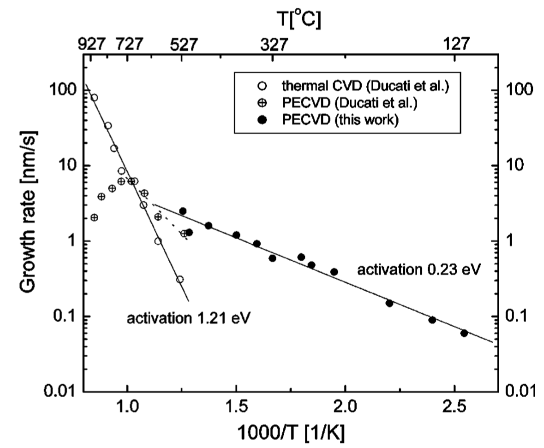
\includegraphics[width=8cm]{src/fig/fig38.png}
\caption{The activation energy in thermal-CVD and PE-CVD\textsuperscript{[22]}}
\end{figure}
With the assist of Hofmann’s low-temperature experiment result, we can get the essential rate constant values by fitting. 
\begin{figure}[H]
\centering
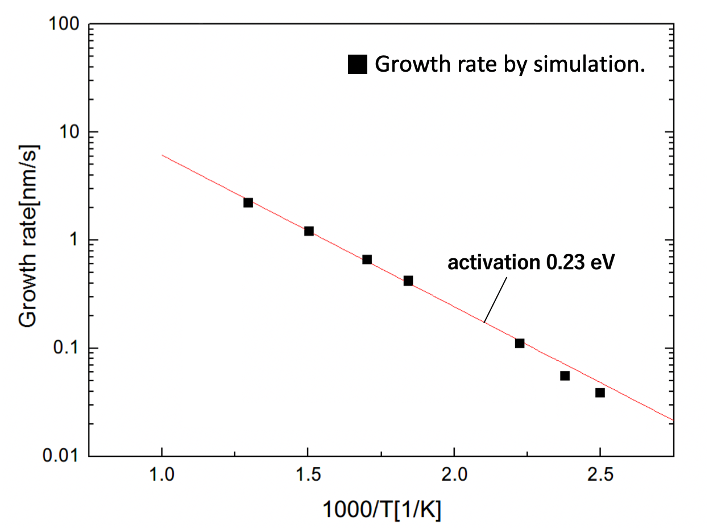
\includegraphics[width=8cm]{src/fig/fig39.png}
\caption{The fitted growth rate}
\end{figure}
Comparing the growth rates in fig. 3.9 (experimental result) and fig.3.10 (fitting result) the credibility of this CNT modeling is confirmed. It should be mentioned that in low-temperature region,  simulated length will be shorter than experiment result for the cone structure of CNF at lower temperature. Such deviation is because this calculation model assume  the tube shape, so $z$ ,the carbon atoms per meter in CNT will be larger than that in cone shape. 

\subsection{Ni silicidation\textsuperscript{[42]}}
There are tremendous investigation  into Ni silicidation in the field of electronic device. As we know, at a given high temperature, Ni silicidation occurs. Although Silicon atom is highly mobile, it is widely reported that that it is Ni atoms that being the dominant diffusing species in the phases in the Ni–Si system\textsuperscript{[43]}. According to Ni–Si binary phase, interphases including $\mathrm{Ni_{2}Si}$, $\mathrm{NiSi}$, $\mathrm{NiSi_{2}}$, $\mathrm{Ni_{5}Si_{2}}$ , $\mathrm{Ni_{3}Si}$ exist. However, the sequence of phases formed during silicidation does not necessarily follow the respective equilibrium diagrams, that is to say, some intermediate phases might be missing. Besides, in a low temperature range (200$\sim$325\(^\circ\)C), only $\mathrm{NiSi_{2}}$ exist on Si wafer, indicating that $\mathrm{NiSi_{2}}$ is the initial phase if at a higher temperature where Ni can proceed deeper in Silicon. With temperature increasing (300$\sim$400\(^\circ\)C), $\mathrm{NiSi}$  starts to form, followed by $\mathrm{NiSi_{2}}$ . The reaction kinetics of formation of the new phase can be categorized in to two (i) diffusion, (ii) nucleation. The formation of $\mathrm{Ni_{2}Si}$ and $\mathrm{NiSi}$ are diffusion-controlled while $\mathrm{NiSi_{2}}$  is nucleation controlled. 
Here we treat the Ni-silicidation issue based on the Fick’s law.

First, several assumptions are made to simplify the calculation. 
\begin{enumerate}[(i)]
\item Ni diffuses into Si.
\item One dimension diffusion.
\item Semi-infinite diffusion.
\item Only $\mathrm{Ni_{2}Si}$  phase is formed at T<300\(^\circ\)C
\end{enumerate}
\begin{figure}[H]
\centering
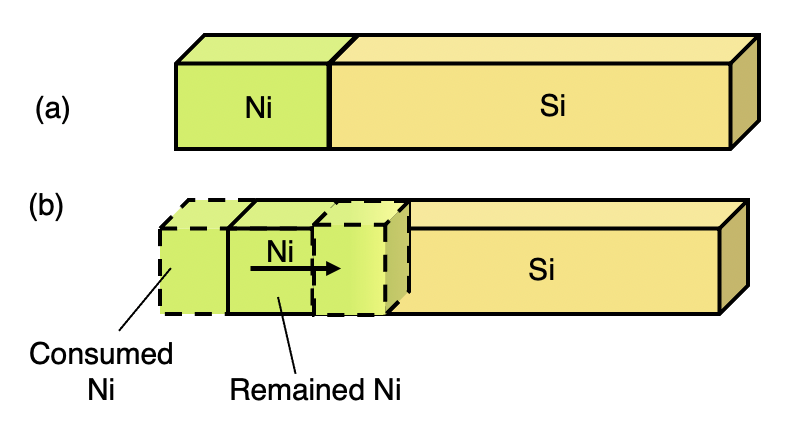
\includegraphics[width=8cm]{src/fig/fig40.png}
\caption{The one-dimension silicidation model at (a)initial, (b)in the process of annealing.}
\end{figure}
The diffusion coefficient $D$ of Ni is defined as,
\begin{equation}
D=D_{0} \exp \left(-E_{a} / k_{B} T\right)
\tag{3.2.18}
\end{equation}
Using the reported value $D= 2 \times 10^{-16} cm^{2}/sec$ at 200$^{\circ}$C and $E_{a}=1.5 eV$\textsuperscript{[42]}. Assume $D_{0}$ is constant at T<300$^{\circ}$C, thus the value of $D$ at 100$^{\circ}$C and 300$^{\circ}$C can be derived.
%对齐
$$\frac{\partial C}{\partial t}&=D\frac{\partial ^{2}C}{\partial x^{2}}$$
\begin{equation}
\begin{array}{lc}
\mathrm{Initial\quad condition}&:\qquad\qquad C(x,0)=0 \\
\mathrm{Boundary\quad condition\quad I}&:\qquad\qquad C(0,t)=C_{0}\\
\mathrm{Boundary\quad condition\quad I\hspace{-1pt}I}&: \qquad\qquad C(d_{Si},t)=0
\end{array}
\tag{3.2.19}
\end{equation}
General solution:
\begin{equation}
C(x, t)=C_{0} \operatorname{erfc}(x/2 \sqrt{D t})
\tag{3.2.20}
\end{equation}
Thus the concentration profile of Ni in Si is obtained. The integration of $C(x,t)$ from $0$ to $d_{Si}$ at certain moment(e.x. $t=1$ min) is the total consumption of Ni at that moment. By applying increasing $t$ into this integration eqaution the Ni consumption variation is obtained. The exact number of Ni atoms diffused into Si is not our interest but the relative ratio of remained Ni to initial Ni. If at the end of annealing there is still some pure Ni on the surface of Si particle, it's can be seen that the Ni is active as a catalyst. In the case of Ni:Si-NP, the size of Si is 20nm. The annealing time in PE-CVD is 15 minutes. 
\newpage
\subsection{Simulation result }
\begin{figure}[H]
\centering
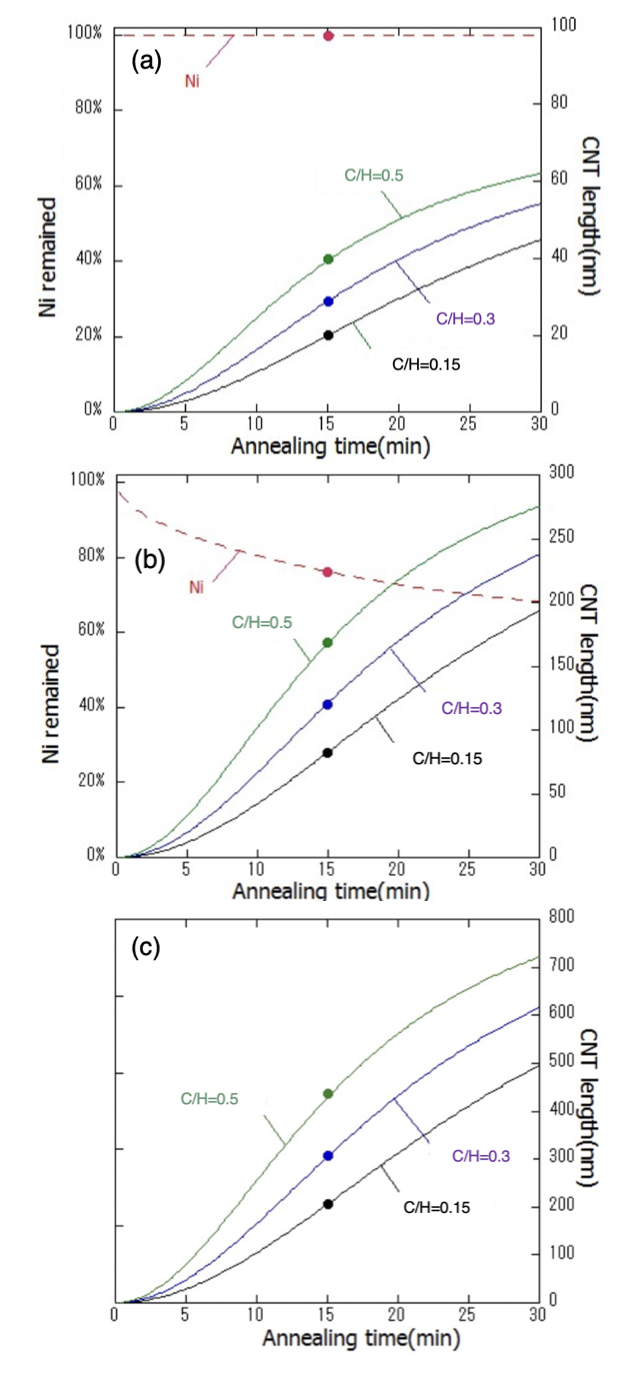
\includegraphics[width=8cm]{src/fig/fig41.png}
\caption{Competitive process between CNT growth and Ni silicidation at different annealing temperature of (a)100\(^\circ\)C (b)200\(^\circ\)C (c)300\(^\circ\)C}
\end{figure}

Except for temperature, another parameter that is controlled in this experiment is gas ratio. Due to the complexity of treating plasma, we assume that only temperature influence Ni silicidation. As to CNT calculation, It should be noted that gas ratio do influence the CNT growth for that the partial pressure of $\mathrm{C_{2}H_{2}}$ is changed. In addition, The gas ratio influence CNT growth in a way of changing  the  H species which is provide by $\mathrm{NH_{3}}$, however, not taken into this calculation due to the difficulty to quantify. The function of $\mathrm{NH_{3}}$ is to etch the competing amorphous carbon and graphitic phases. It may also have a role in keeping the gas side of the catalyst particle free of carbon, to allow continuing access of gas to the catalyst, and prevent it from becoming deactivated. While the flowrate of $\mathrm{NH_{3}}$ is changed to control the gas ratio, the plasma properties remains basically the same due to constant pressure.
\begin{table}[H]
\centering
\caption{Denotation of gas ratio}
\begin{tabular}{cc}
\toprule
Flow rate(sccm) & Denotation \\ \midrule
$\mathrm{C_{2}H_{2}}:\mathrm{NH_{3}=14:70}$ & C/H=0.15     \\
$\mathrm{C_{2}H_{2}}:\mathrm{NH_{3}=14:35}$ & C/H=0.3     \\
$\mathrm{C_{2}H_{2}}:\mathrm{NH_{3}=14:14}$ & C/H=0.5     \\ \bottomrule
\end{tabular}
\end{table}
Assuming CNT growth and Ni silicidation are independent from each other. On a Si nanoparticle($d_{Si}=20 nm$) with a grafted Ni cap($r_{Ni}=5 nm$)  we have the simulation result as fig.3.12 shows. At 100\(^\circ\)C, Ni silicidation is not occurring but due to the low temperature and the growth rate of CNT is suppressed as well. At 200\(^\circ\)C Ni silicidation occurs and CNT grows relatively faster. After annealing, the 300nm-long-CNT is grown and around 20\% of Ni cap is consumed. Unfortunately, when calculating the 300℃ case, Ni diffuse too fast that no longer meet the assumption of semi-finite diffusion.  





\chapter{Result \& Discussion}
\section{Powder characteristics}
\subsection{Size distribution}
According to previous research, the nanoparticles with a size of tens of nanometers are defined as primary particles,  the particles with the size of 0.1 to 1 $\mathrm{\mu m}$ are defined as secondary particle, and likewise, those particles with larger sizes are defined as tertiary and quaternary particles.
As Fig. 4。1 shows, it is confirmed that the pure Si nanoparticles exhibit a large bump from 0.1 to 10 µm and major of them are within 1 to 10 $\mathrm{\mu m}$. The size distribution of pure Si nanoparticles  is uniform. On the other hand, with Ni addition, there are two major peaks with the center around 0.1 $\mathrm{\mu m}$ and 10~20 $\mathrm{\mu m}$, which indicates that the Ni addition induce partly agglomeration of nanoparticles. 
\begin{figure}[H]
\centering
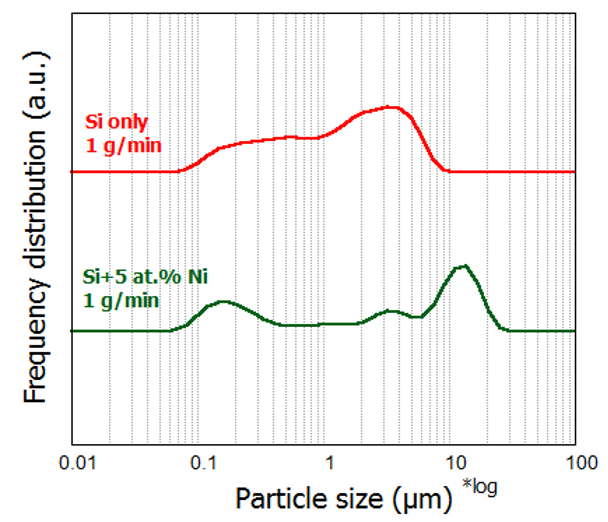
\includegraphics[width=8cm]{src/fig/fig42.png}
\caption{Particle size distribution.}
\end{figure}
\newpage
\subsection{Particle morphology}
The surface morphologies of the PS-PVD processed Si nanocomposites with and without Ni addition  is revealed by SEM. As figure 4.2 shows,  the raw mg-Si powder is about 20 µm on average and in a sharp-cornered shape. In contrast, the size of PS-PVD processed nanoparticles are significantly reduced and exhibits a more spherical shape. Due to limited amount of Ni addition, the morphology of processed Si:Ni nanoparticles are similar to that of Si-only nanoparticles, samely reduced size and spherical shape. That is, the 5 at.\% Ni addition can not make significantly change to nanoparticle morphology.
\begin{figure}[h]
\centering
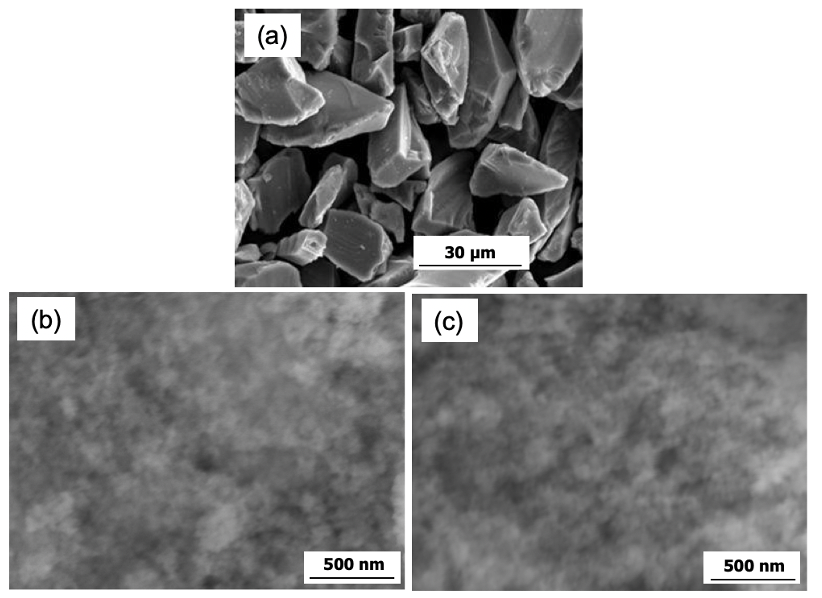
\includegraphics[width=12cm]{src/fig/fig43.png}
\caption{SEM micrograpghs of  PS-PVD processed powders (a) raw powder(MG-Si); (b) Si-only particles; (c) Si:Ni particles}
\end{figure}
\begin{figure}[h]
\centering
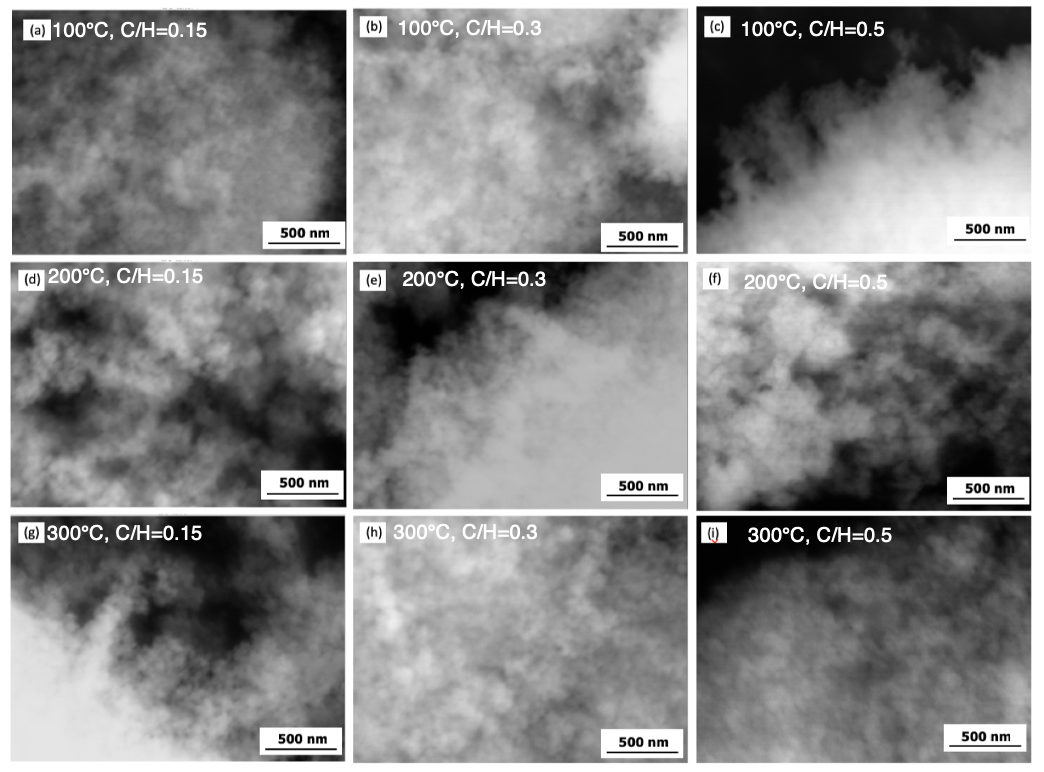
\includegraphics[width=12cm]{src/fig/fig44.png}
\caption{SEM images of PE-CVD post annealed nanopowders at different temperature and gas ratios}
\end{figure}

Figure 4.3 shows the SEM micrograpghs of the PE-PVD post annealed Si:Ni nanoparticles at different temperature and gas ratios. It’s clear that the post-annealing has not significantly change the morphology of nanoparticles. Unfortunately, the rod-like materials is not found. 

The possible reasons might be: 
\begin{itemize}
  \item Carbon nanotubes do grow, but are to short or hidden in this cotton-like nanostructure to be distinguished due to limited resolution of SEM.
  \item Carbon nanotubes is not grown, instead, carbon deposited on Si:Ni-NPs in the form of amorphous carbon, which is inferred by EDS analysis. 
\end{itemize}
\newpage
Figure 4.4 the EDS mapping illustrates the distribution of elements in PE-CVD post annealed powders. It’s clear that the major element is Si, and other elements like Ni, C and O are uniformly distributed on Si nanoparticles. The EDS energy spectrum also reveal the presence of carbon in a qualitative way. The presence of Oxygen feature is probably due to an exposure of the samples to air.
\begin{figure}[H]
\centering
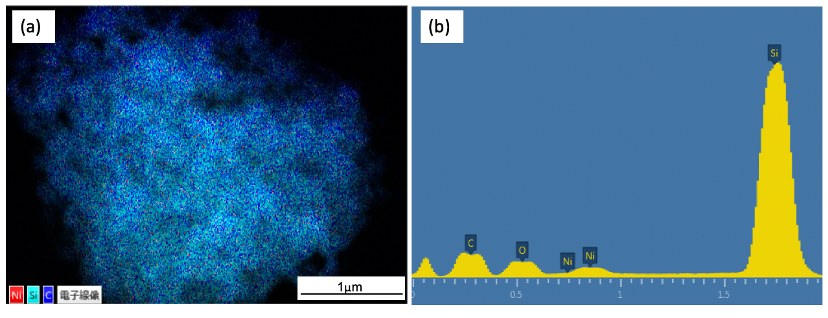
\includegraphics[width=12cm]{src/fig/fig45.png}
\caption{(a) Si, C, Ni, and O element mapping by EDS. (b)element content.}
\end{figure}
\newpage
%拉曼
\subsection{Raman spectroscopy}
Figure 4.6 shows the Raman spectroscopy of 200\(^\circ\)C annealed powder with different gas ratio. In the range of 200 to 1800 $\mathrm{cm^{-1}}$, only the peak responsible for crystalline Si exist(500\(^\circ\)). Especially around 1380 $\mathrm{cm^{-1}}$ (D peak) and 1600 $\mathrm{cm^{-1}}$(G peak), the intensity is close to zero. It implies that the carbon nanotubes is not successfully grown.  
\begin{figure}[h]
\centering
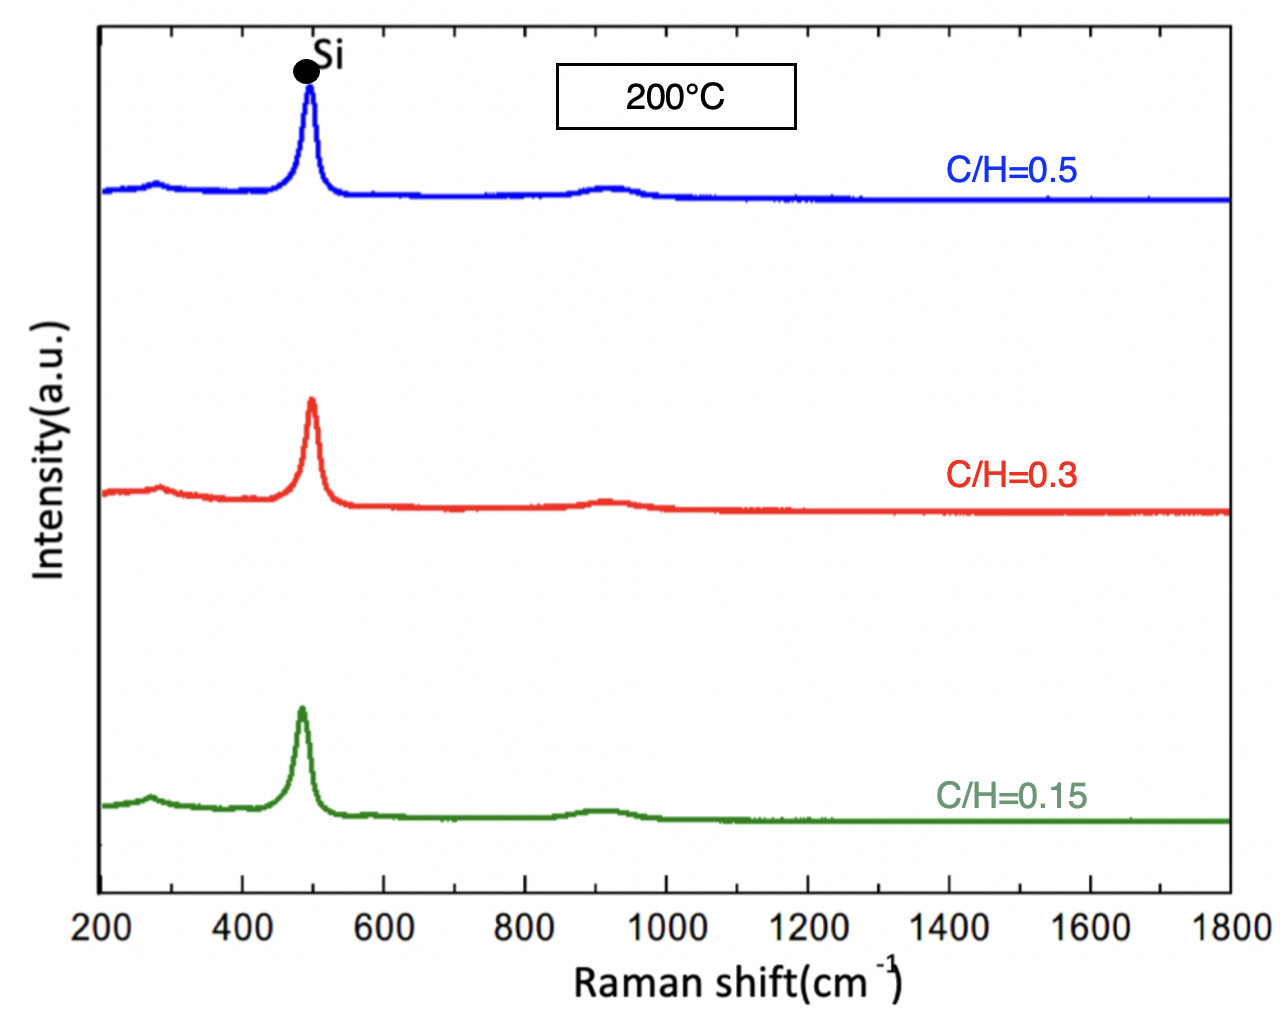
\includegraphics[width=8cm]{src/fig/fig46.png}
\caption{Raman spectroscopy of annealed Si:Ni powders at 200\(^\circ\)C}
\end{figure}
%XRD
\subsection{Phase analysis}
\begin{figure}[h]
\centering
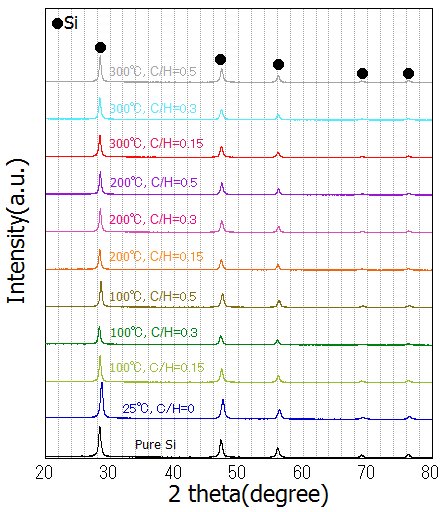
\includegraphics[width=8cm]{src/fig/fig47.png}
\caption{XRD pattern of powders}
\end{figure}
The deference in XRD patterns of annealed powders at different temperature and gas ratio is indistinct. Due to small amount of Ni addition and relatively low temperature annealing, even $\mathrm{Ni_{x}Si}$ phase exist. It’s difficult to distinguish with comparison to the towering Si peak.
\begin{table}[H]
\caption{Rietveld analysis of silicidation at different temperature}
\begin{tabular}{ccccccc}
\toprule
\begin{array}{c}
\text {Temperature} \\
\text {(\(^\circ\)C)}
\end{array}  &  
\begin{array}{c}
\text {Si } \\
\text {(at.\%)}
\end{array}&
\begin{array}{c}
\text {$\mathrm{NiSi_{2}}$} \\
\text {(at.\%)}
\end{array}    & 
\begin{array}{c}
\text {$\mathrm{NiSi}$} \\
\text {(at.\%)}
\end{array}    &  
\begin{array}{c}
\text {$\mathrm{Ni_{2}Si}$} \\
\text {(at.\%)}
\end{array}    & 
\begin{array}{c}
\text {Ni} \\
\text {(at.\%)}
\end{array}  & \begin{array}{c}
\text {Ni Remained} \\
\text {(at.\%)}
\end{array} 
\\ \midrule
25 & 96.45 & 0.90 & 0.70 & 0.88 & 1.06 & 100.00       \\
10& 96.02 & 1.49 & 0.99 & 0.61 & 0.90 & 84.56     \\
200 & 96.13 & 1.35 & 1.12 & 0.72 & 0.68 & 64.26     \\
300 & 94.68 & 2.17 & 1.73 & 1.20 & 0.26 & 24.56     \\ \bottomrule
\end{tabular}
\end{table}
The degree of  Ni silicidation is quantified in the way of considering the relative amount of pure Ni before and after annealing. It’s believed that the gas ratio is of little effect to Ni silicidation, so the Rietveld analysis result is carried out among powders with fixed gas ratio(C/H=0.15). Dividing the amount of Ni after annealing by that of Ni before annealing(RT), the percentage of unconsumed Ni amount is obtained. Compare this result to simulation, for 100\(^\circ\)C case, the simulation suggests no silicidation occurs. But from Rietveld analysis result, silicidation consumes about 15 at.\% of Ni. Additionally, at 200\(^\circ\)C, the simulation shows $\sim$ 75 at.\% is remain unconsumed and Rietveld analysis shows 84.56 at.\%. At 300\(^\circ\)C, the simulation shows it’s limit that it’s not applicable to  higher temperature. But the Rietveld analysis demonstrate the relatively serious Ni silicidation for about 80 at.\% Ni atoms are involved in.
\begin{figure}[H]
\centering
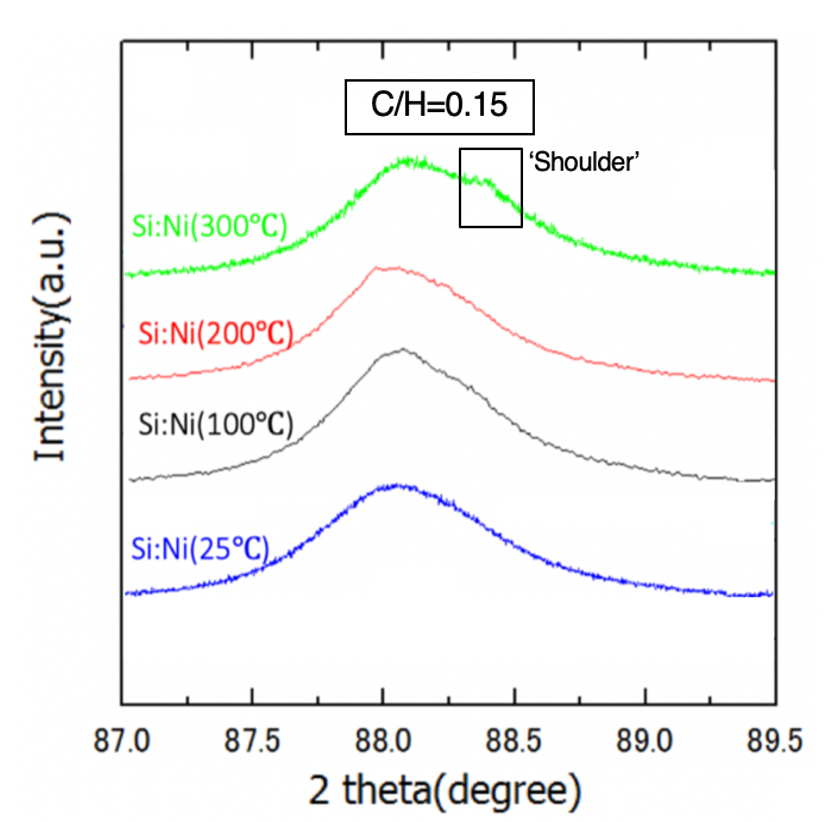
\includegraphics[width=8cm]{src/fig/fig48.png}
\caption{High angle(87$\sim$90\(^\circ\)) XRD pattern of powders at different temperature with a fixed gas ratio of C/H=0.15}
\end{figure}
From figure 4.7, it’s clear that the high angle XRD pattern of 25\(^\circ\)C, 100\(^\circ\)C, 300℃\(^\circ\)C are similarly shaped. But the 300\(^\circ\)C powders exhibit a shoulder around 88.4\(^\circ\). Thus peak fitting was performed using Origin Pro in Origin Lab. The two theta values used for distinguish silicide peaks are:
$$ \mathrm{Si}: 88.029^{\circ} \qquad  \mathrm{NiSi_{2}}: 88.390^{\circ}\qquad  \mathrm{Ni_{2}Si}: 88.673^{\circ}\qquad \mathrm{ NiSi}: 88.796^{\circ}$$
\begin{figure}[H]
\centering
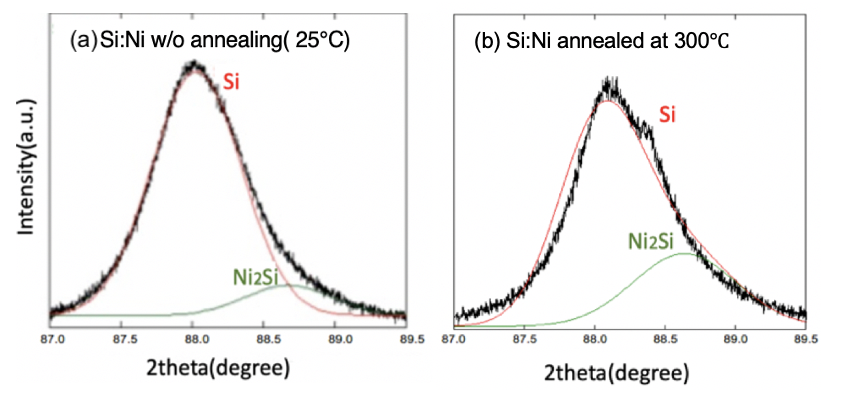
\includegraphics[width=12cm]{src/fig/fig49.png}
\caption{peak fitting of Si:Ni particles (a)without annealing  and (b)  annealed at 300\(^\circ\)C }
\end{figure}
The peak fitting result shown in figure 4.8 indicates an increase of $\mathrm{NiSi_{2}}$ phase content after annealing at 300\(^\circ\)C, further confirms that such right-shifted shoulder is due to Ni silicide. \\
\subsection{Si carbonous structure by TEM}
\begin{figure}[H]
\centering
\includegraphics[width=8cm]{src/fig/fig50.png}
\caption{FE-TEM image of Si:Ni:C nanoparticle}
\end{figure}
The TEM image further confirms the nanostructure in which Ni cap is directly attached on the Si nanoparticle. The diameter of Si is 20$\sim$30 nm and the size of radius of Ni is $\sim$10 nm. From figure 4.9, it’s seen that the particle is encapsulated in an amorphous coating with a uniform thickness of $\sim$3 nm. Figure. 4.9(b) and (d) shows the existence of crystalline part in amorphous carbon coating. Especially in (b), the rod extruded from Ni surface is inferred to be the nuclei of CNT.  From figure (c), it’s clear that the Ni silicidation takes place and almost the entire Ni transformed into $\mathrm{Ni_{2}Si}$ phase. 
  
Since it’s confirmed by TEM observation that amorphous carbon coating forms on Si:Ni:C-NP surface instead of CNT. Still, we can use the same mathematics model to calculate the thickness of amorphous carbon coating.  The length of CNT at different growth condition is obtained by simulation. With known the areal density of carbon and the carbon atomic radius, the convert the CNT length into thickness. 
\begin{center}
    &\text { Table. } 4.2 \text { Length of CNT and thickness of a-C coating }
\end{center}
$$
\begin{aligned}
&\begin{array}{|c|c|c|c|c|c|c|c|c|c|}
\hline \text { Temperature }\left({ }^{\circ} \mathrm{C}\right) & \multicolumn{3}{|c|} {100} & \multicolumn{3}{|c|} {200} & \multicolumn{3}{|c|} {300} \\
\hline \text { C/H } & 0.15 & 0.3 & 0.5 & 0.15 & 0.3 & 0.5 & 0.15 & 0.3 & 0.5 \\
\hline \begin{array}{c}
\text { Length } \\
\text { of CNT (nm) }
\end{array} & 37.8 & 47.98 & 57.19 & 161.5 & 208.09 & 250 & 410 & 535.5 & 655 \\
\hline \begin{array}{c}
\text { Thickness } \\
\text { of a-C coating(nm) }
\end{array} & 0.6 & 0.761 & 0.907 & 2.56 & 3.3 & 3.98 & 6.5 & 8.49 & 10.4 \\
\hline
\end{array}
\end{aligned}
$$
 The thickness  of a-C coating observed by TEM is 3 nm and according to simulation it should be 10.4 nm. The possible reason accounts for this phenomenon are as follows. First, the mathematics model assume flowing $\mathrm{C_{2}H_{2}}$ is totally decomposed, which in general difficult. Second,   the NH3  etching effect is ignored. So simulation usually get a larger value of product. It’s reasonable that the actual thickness is smaller than simulated thickness.
 \newpage
 \section{Battery performance}
 It's known that amorphous carbon coating can improve the specific capacity of Si nanoparticles due to its flexibility and enhance electrical conductivity. As for the Ni silicide formed during annealing, since it consumes part of Si, it reduces the theoretical capacity. 
・reduce resistance
\begin{figure}[H]
\centering
\includegraphics[width=8cm]{src/fig/fig51.png}
\caption{The specific capacity of annealed Si:Ni:C-NP in 30 cycles}
\end{figure}
\begin{figure}[H]
\centering
\includegraphics[width=8cm]{src/fig/fig52.png}
\caption{The impedance of annealed Si:Ni:C-NPs}
\end{figure}

\subsubsection{C/H dependence}
\noindent $\bullet$ Specific capacity\\
According to figure 4.10, at 300\(^\circ\)C the specific capacity sequence is: 
$$\mathrm{[C/H=0.3] > [C/H=0.5] > [C/H=0.15]}$$
This is because the silicidation of  all Si:Ni:C-NP annealed at 300\(^\circ\)C is so serious, but Si:Ni:C with thicker carbon coating exhibits the best structural integrity and highest specific capacity. Or it might be that the much H radical in plasma etches away all carbon deposition on surface, the final product is as same as undeposited one  On the other hand, Si:Ni:C-NP with higher $\mathrm{NH_{3}}$ concentration so that the carbon coating is too thin to provide buffering effect. Compared to w/o annealing Si:Ni-NP, the capacity is even lower. As for Si:Ni:C-NP with C/H=0.5, as shown in TEM, is covered with a uniform a-C coating and within the coating there is segment of crystalline carbon. So the capacity is in between. It has been reported that C/H-0.3 is expected to be the optimal ratio to grow CNTs. We postulate that the deposition product of C/H=0.3 case is a mixture of CNTs and a-C coating based on the TEM image of C/H=0.5 case. But the CNTs are too short and the content of crystalline C is too low to be detected by Raman spectroscopy. The short CNTs can connect to other particles and form a matrix to provide better buffering effect than pure a-C coating.\\
\noindent $\bullet$ Conductivity\\
According to figure 4.11, at 300\(^\circ\)C the conductivity sequence is: 
$$\mathrm{[C/H=0.5] > [C/H=0.3] > [C/H=0.15]}$$
Similarly, the Si:Ni:C-NP with C/H=0.15 has the largest impedance due to the silicidation and low carbon content. And, the Si:Ni:C-NP with C/H=0.5 exhibits the smallest impedance due to the highest carbon content.
\subsubsection{Temperature dependence}
\noindent $\bullet$ Specific capacity\\
According to figure 4.10, at C/H=0.3 the specific capacity sequence is: 
$$\mathrm{[300^{\circ}C]> [200^{\circ}C] > [100^{\circ}C]}$$
Basically the higher temperature the higher capacity. At 100\(^\circ\)C and 200\(^\circ\)C, the silicidation is slightly, at 200\(^\circ\)C the carbon coating is thicker so capacity will be improved compared to 200\(^\circ\)C. At 300\(^\circ\)C the silicidation is serious but still the capacity is improved compared to 200\(^\circ\)C due to the thicker carbon coating. It's inferred that the positive effect provided by a-C coating is dominant when silicidation occurs. \\
\noindent $\bullet$ Conductivity\\
According to figure 4.11, at C/H=0.3 the conductivity sequence is: 
$$\mathrm{[300^{\circ}C]> [200^{\circ}C] > [100^{\circ}C]}$$
At the optimal C/H ratio of 0.3, the impedance is purely depended on the silicidation.
The slighter silicidation, the better conductivity.
%\newpage

\chapter{Conclusion}
The present study was carried out aiming to fabricate novel Silicon-based anode  for next-generation LIBs.  To attain high energy density, Silicon should be nano-sized to prevent its rapid volume expansion, carbonous materials are often used as additives to buffer the volume change as well as enhance the conductivity. Among all carbonous materials, carbon nanotubes is the material of interest for it’s large aspect ratio and high electrical conductivity. The method to fabricate nano-sized Silicon is PS-PVD for the high throughput and the feasibility of industrial-scale production. To make full use of the Si:Ni nanostructure where Ni directly attached on Si nanoparticle, a low-temperature CNT growth method was utilized. 

In this study,
\begin{enumerate}[(1)]
\item A low-temperature CNT growth mathematical model was established.
\item The competitive process between Ni silicidation and carbon deposition was simulated. By modeling the CNT growth and Ni silicidation, the proper experimental condition was set.
\item However, the experimental result reveals that the product of annealing is a uniform carbonous coating instead of CNT. Still, the mathematical model is ready to simulate the carbon coating thickness.
\item The correlation between silicide, amorphous carbon coating and battery performance was evaluated. There is a trade-off: the higher temperature, the more carbonous product on Si:Ni-NP surface to increase capacity. But the Ni silicidation is also promoted, which consumes Si, then decrease the capacity. And Ni silicide decrease conductivity of battery as well.
\end{enumerate}

So far, the CNT growth mechanism remains unclear,  and introducing plasma add up the complexity to quantify CNT growth. PE-CVD of CNTs is an extremely complex process with numerous coupled phenomena: plasma chemistry, neutral and ion reactions, surface chemistry, catalyzed growth, catalyst particle aggregation and poison, additional plasma heating, electric field effects, ion bombardment. The model established in this study use only major two parameters: Temperature and carbon concentration. Although the initial purpose is to grow CNT at low temperature, this model and simulation is applicable for other forms of carbon. 

\chapter{Acknowledgements}
I  wish to express my sincere appreciation to my supervisor, Professor Kambara, who has provided much patient and offered useful guidance on this research.  I still remember the assistant and tips  he gave me while working together to  build the  PE-CVD apparatus. 

Thanks also to my tutor Ohta, for the abundant knowledge sharing with me. He has ffered much help on my study. 

Thanks my mates: Kusumoto, Ishbashi, Sumi, Hamasaki, Murata, Miki, Hiraoka. 

Thank you all for your support and patience. 
       

\end{document}
